\documentclass[professionalfonts, xcolor=table]{beamer}
%% \documentclass[professionalfonts, xcolor=table, handout]{beamer}
%% \usepackage{pgfpages}
%% \pgfpagesuselayout{4 on 1}[a4paper,border shrink=5mm, landscape]
\usepackage{fontspec}
\usepackage{amsmath,amssymb}
\usepackage{tikz}
\usetikzlibrary{positioning, matrix, arrows.meta, shapes.geometric,
  decorations.pathmorphing, decorations.pathreplacing, fit, shapes.multipart}
\usepackage{mathabx}
\usepackage{mathtools}
\usepackage{mathpartir}
\usepackage{fancyvrb}
\usepackage{stmaryrd}
\usepackage[absolute,overlay]{textpos}

\defaultfontfeatures{Mapping=tex-text,Scale=MatchLowercase}
%\setmainfont{Palatino}
%\setsansfont{Helvetica}
%\setmainfont{Minion Pro}
%\setsansfont{Myriad Pro}
%\setmonofont{Menlo Regular}
\usetheme{CambridgeUS}

\definecolor{lightg}{RGB}{217,232,225}
\definecolor{darkg}{RGB}{6,81,42}

\useinnertheme{circles}
\setbeamertemplate{enumerate item}[default]
\usecolortheme{spruce}
\usefonttheme{serif}
\setbeamerfont*{frametitle}{series=\bfseries}
\setbeamercolor{alerted text}{fg=red}
\setbeamertemplate{navigation symbols}{}
\setbeamercolor{emphC}{fg=red}
\setbeamercolor{block title}{bg = darkg, fg=white!80}
\setbeamercolor{block body}{bg = lightg, fg=black}

\newcommand{\scon}{\mathbin{\varstar}}
\newcommand{\ocon}{%
  \mathbin{\mbox{$\mathrlap{\cup}\hspace*{.15em}
      \raisebox{.01em}[0ex][0ex]{$\scon$}$\hspace*{.07em}}}}
\newcommand{\medocon}{
  \raisebox{-0.3ex}{\resizebox{0.63em}{!}{$\scon$}} \hspace{-2.4ex} \bigcup}
\newcommand{\wand}{%
 \mathrel{\mbox{$\hspace*{-0.03em}\mathord{-}\hspace*{-0.66em}
  \mathord{-}\hspace*{-0.36em}\mathord{\scon}$\hspace*{-0.005em}}}}
\newcommand{\defeq}{\mathbin{\overset{\mathrm{def}}{=}}}
\newcommand{\emphd}[1]{{\bfseries #1}}
\newcommand{\emphr}[2]{\alert<#1>{#2}}
\newcommand{\bracket}[1]{[#1]}
\makeatletter\let\frametextheight\beamer@frametextheight\makeatother
\newcommand\credit[1]{%
  \begin{textblock*}{\paperwidth}(0pt,\textheight)
    \raggedleft #1\hspace{.5em}
\end{textblock*}}
\newcommand{\pguards}[1]{\llbracket #1 \rrbracket}

\title[Mechanized Verification]{Mechanized Verification of \\
  Graph-manipulating Programs}
\author[Wang, Cao, Mohan, Hobor]{Shengyi Wang, Qingxiang Cao, Anshuman Mohan, \underline{Aquinas Hobor}}
\institute[NUS]{National University of Singapore}
\date{\today}
%% \setbeamercovered{transparent}
\begin{document}
\begin{frame}
  \titlepage
\end{frame}

\newcommand\hide[1]{}

\section{Motivation}

%\hide{

\begin{frame}{Our Focus}
We would like to verify \alert{graph-manipulating} programs written in \alert{real C}
with end-to-end \alert{machine-checked} correctness proofs.
\begin{itemize}
\item Graph algorithms are hard to reason about but occur in critical areas of real systems
\item Real C code has achingly subtle semantics in some places
\item Machine-checked proofs are merciless and lengthy: we want to reuse existing codebases
\end{itemize}
\end{frame}

\begin{frame}{Our Strategy}
We will use the \alert{CompCert} certified compiler's definition of C and the \alert{Verified Software Toolchain}'s (VST) version of \alert{Separation Logic} to certify our code against strong specifications expressed with \alert{mathematical graphs}.
\begin{itemize}
\item Between them, CompCert and VST have 50+ person-years worth of development effort.  \alert{It is highly desirous to fit within their frameworks rather than reinventing the wheel.}
\item We make no changes to CompCert.  We make minimal (\alert{approximately 1\% of codebase}) additions to VST (two new tacticals, assorted lemmas).
\item Our techniques use vanilla separation logic (albeit with $\wand$ and quantifiers).
\item We have developed an expressive machine-checked framework for mathematical graphs that is \alert{powerful enough to verify real code}.
\end{itemize}
\end{frame}


\begin{frame}{Our Results}
We have verified half a dozen graph algorithms, including:
\begin{itemize}
\item Graph visiting/coloring; ditto for DAG
\item Graph reclamation (\emph{i.e.} spanning tree followed by tree reclamation)
\item Union-find (both for heap- and array-represented nodes)
\item Garbage collector for CertiCoq project
\begin{itemize}
\item Generational OCaml-style GC for a purely functional language
\item $\approx$400 lines of (rather devilish) C
\item We pinpoint two places where C is too weak to define an OCaml-style GC
\item Verify (almost) full graph isomorphism
\item $\approx$14,000 lines of example-specific proof script
\end{itemize}
\end{itemize}
\end{frame}

\begin{frame}{Union-Find Algorithm}
  \centering
  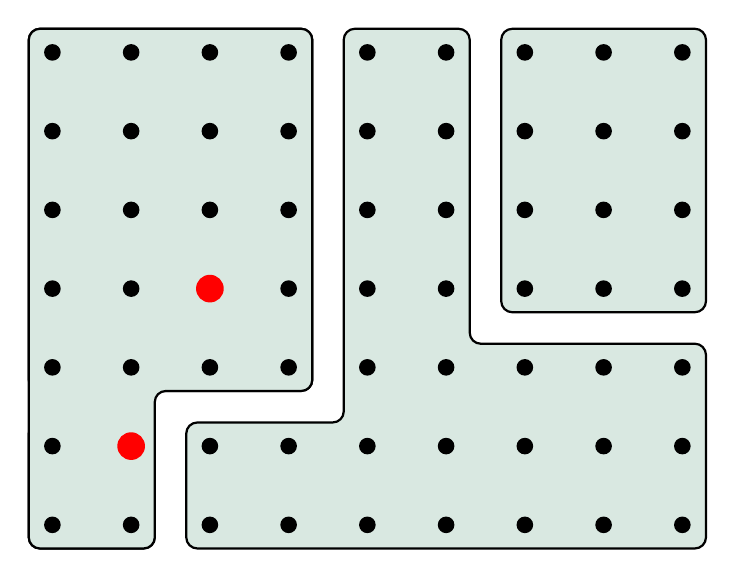
\begin{tikzpicture}[rounded corners]
    \uncover<2,3>{\draw[thick, fill=lightg] (-0.3, -0.3) rectangle (1.3, 1.3);}
    \uncover<2,3>{\draw[thick, fill=lightg] (-0.3, 1.7) rectangle (3.3, 6.3);}
    \uncover<2->{\draw[thick, fill=lightg] (5.7, 2.7) rectangle (8.3, 6.3);}
    \uncover<2->{\draw[thick, fill=lightg] (1.7, -0.3) -- (8.3, -0.3) -- (8.3, 2.3) --
      (5.3, 2.3) -- (5.3, 6.3) -- (3.7, 6.3) -- (3.7, 1.3) -- (1.7, 1.3) -- cycle;}
    \draw<4->[thick, fill=lightg] (-0.3, -0.3) -- (1.3, -0.3) -- (1.3, 1.7) --
    (3.3, 1.7) -- (3.3, 6.3) -- (-0.3, 6.3) -- cycle;
    \foreach \x in {0, ..., 8}
    \foreach \y in {0, ..., 6}
    \fill[black] (\x, \y) circle (3pt);
    \fill<3->[red] (1, 1) circle (5pt);
    \fill<3->[red] (2, 3) circle (5pt);
  \end{tikzpicture}
\end{frame}

\begin{frame}[fragile]{Union-Find Algorithm: Disjoint-Set Data Structure}
  \begin{columns}[c]
    \column{.4\textwidth}
    \centering
    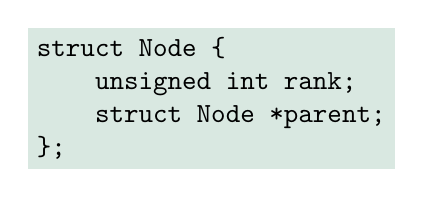
\begin{tikzpicture}
      \node [rectangle, fill=lightg] {
\begin{BVerbatim}[commandchars=\\\[\]]
\emphd[struct] Node {
    unsigned int rank;
    \emphd[struct] Node *parent;
};
\end{BVerbatim}
      };
    \end{tikzpicture} \pause
    \column{.6\textwidth}\centering
    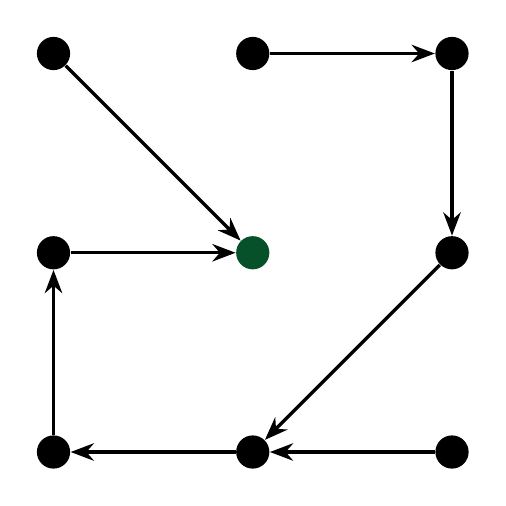
\begin{tikzpicture}[
        gn/.style={circle, inner sep=0pt, minimum size=12pt, fill=black},
        rn/.style={circle, inner sep=0pt, minimum size=12pt, fill=darkg},
        ->/.style={-Stealth, very thick}]
      \matrix[row sep=60, column sep=60]{
        \node[gn] (g1) {}; & \node[gn] (g2) {}; & \node[gn] (g3) {};\\
        \node[gn] (g4) {}; & \node[rn] (g5) {}; & \node[gn] (g6) {};\\
        \node[gn] (g7) {}; & \node[gn] (g8) {}; & \node[gn] (g9) {}; \\
      };
      \draw [->] (g1) to (g5);
      \draw [->] (g2) to (g3);
      \draw [->] (g3) to (g6);
      \draw [->] (g6) to (g8);
      \draw [->] (g9) to (g8);
      \draw [->] (g8) to (g7);
      \draw [->] (g7) to (g4);
      \draw [->] (g4) to (g5);
    \end{tikzpicture}
  \end{columns}
\end{frame}

\begin{frame}[fragile]{Union-Find Algorithm: Find}
  \begin{columns}[c]
    \column{.6\textwidth}
    \centering
   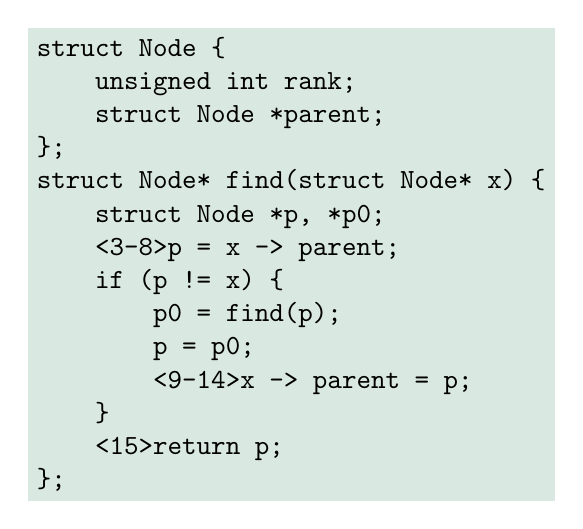
\begin{tikzpicture}
      \node [rectangle, fill=lightg] {
\begin{BVerbatim}[commandchars=\\\[\]]
\emphd[struct] Node {
    unsigned int rank;
    \emphd[struct] Node *parent;
};
\emphd[struct] Node* find(\emphd[struct] Node* x) {
    \emphd[struct] Node *p, *p0;
    \emphr[3-8][p = x -> parent;]
    \emphd[if] (p != x) {
        p0 = find(p);
        p = p0;
        \emphr[9-14][x -> parent = p;]
    }
    \emphr[15][\emphd[return] p;]
};
\end{BVerbatim}
      };
   \end{tikzpicture}
   \column{.4\textwidth}
   \centering
   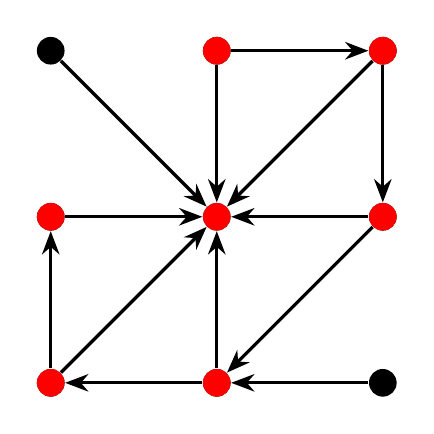
\begin{tikzpicture}[
       gn/.style={circle, inner sep=0pt, minimum size=10pt, fill=black},
       rn/.style={circle, inner sep=0pt, minimum size=10pt, fill=darkg},
       mn/.style={circle, inner sep=0pt, minimum size=10pt, fill=red},
       ->/.style={-Stealth, very thick}]
     \matrix[row sep=50, column sep=50]{
       \node[gn] (g1) {}; & \node<1,3-13,15->[gn] (g2) {};
       \node<2,14>[mn] (g2) {}; & \node<1-2,4-12,14->[gn] (g3) {};
       \node<3,13>[mn] (g3) {}; \\
       \node<1-6,8,10->[gn] (g4) {}; \node<7,9>[mn] (g4) {}; &
       \node<1-7,9-14>[rn] (g5) {}; \node<8,15>[mn] (g5) {}; &
       \node<1-3,5-11,13->[gn] (g6) {}; \node<4, 12>[mn] (g6) {}; \\
       \node<1-5,7-9,11->[gn] (g7) {}; \node<6,10>[mn] (g7) {}; &
       \node<1-4,6-10,12->[gn] (g8) {}; \node<5,11>[mn] (g8) {}; &
       \node[gn] (g9) {}; \\
     };
     \draw [->] (g1) to (g5);
     \draw<1-13> [->] (g2) to (g3);
     \draw<14-> [->] (g2) to (g5);
     \draw<1-12> [->] (g3) to (g6);
     \draw<13-> [->] (g3) to (g5);
     \draw<1-11> [->] (g6) to (g8);
     \draw<12-> [->] (g6) to (g5);
     \draw [->] (g9) to (g8);
     \draw<1-10> [->] (g8) to (g7);
     \draw<11-> [->] (g8) to (g5);
     \draw<1-9> [->] (g7) to (g4);
     \draw<10-> [->] (g7) to (g5);
     \draw [->] (g4) to (g5);
   \end{tikzpicture}
  \end{columns}
\end{frame}

\begin{frame}[fragile]{Verifying Graph-Manipulating Algorithm is Hard}
  \begin{center}
    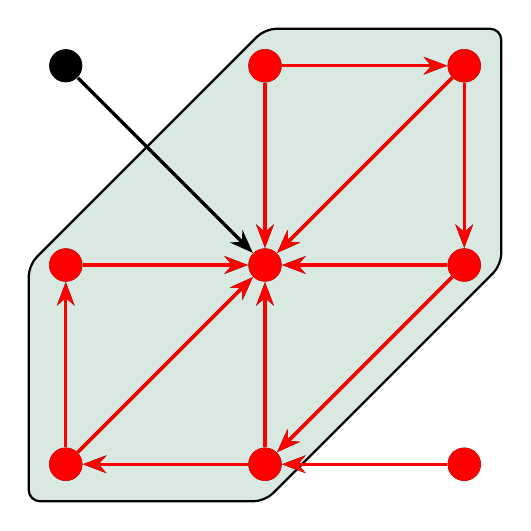
\begin{tikzpicture}[
        gn/.style={circle, inner sep=0pt, minimum size=12pt, fill=black},
        rn/.style={circle, inner sep=0pt, minimum size=12pt, fill=darkg},
        mn/.style={circle, inner sep=0pt, minimum size=12pt, fill=red},
        ->/.style={-Stealth, very thick}]
      \uncover<3->{\draw [fill=lightg, thick, rounded corners] (-3, -3) -- (0, -3) --
        (3, 0) -- (3, 3) -- (0, 3) -- (-3, 0) -- cycle; }
      \matrix[row sep=60, column sep=60]{
        \node[gn] (g1) {}; & \node<1-3,6->[gn] (g2) {}; \node<4-5>[mn] (g2) {}; &
        \node<1-3,6->[gn] (g3) {}; \node<4-5>[mn] (g3) {};\\
        \node<1-3,7->[gn] (g4) {}; \node<4-6>[mn] (g4) {}; & \node<1-3>[rn] (g5) {};
        \node<4->[mn] (g5) {}; & \node<1-3,6->[gn] (g6) {}; \node<4-5>[mn] (g6) {};\\
        \node<1-3,7->[gn] (g7) {}; \node<4-6>[mn] (g7) {}; & \node<1-3>[gn] (g8) {};
        \node<4->[mn] (g8) {}; & \node<1-5>[gn] (g9) {}; \node<6->[mn] (g9) {}; \\
      };
          \draw [->] (g1) to (g5);
          \draw<1,6> [->] (g2) to (g3);
          \draw<4> [->, red] (g2) to (g3);
          \draw<2-3,7-> [->] (g2) to (g5);
          \draw<5> [->, red] (g2) to (g5);
          \draw<1,6> [->] (g3) to (g6);
          \draw<4> [->, red] (g3) to (g6);
          \draw<2-3,7-> [->] (g3) to (g5);
          \draw<5> [->, red] (g3) to (g5);
          \draw<1,6> [->] (g6) to (g8);
          \draw<4> [->, red] (g6) to (g8);
          \draw<2-3,7-> [->] (g6) to (g5);
          \draw<5> [->, red] (g6) to (g5);
          \draw<1-5> [->] (g9) to (g8);
          \draw<6-> [->, red] (g9) to (g8);
          \draw<1> [->] (g8) to (g7);
          \draw<4,6> [->,red] (g8) to (g7);
          \draw<2-3> [->] (g8) to (g5);
          \draw<5,7-> [->,red] (g8) to (g5);
          \draw<1> [->] (g7) to (g4);
          \draw<4,6> [->, red] (g7) to (g4);
          \draw<2-3,7-> [->] (g7) to (g5);
          \draw<5> [->, red] (g7) to (g5);
          \draw<1-3,7-> [->] (g4) to (g5);
          \draw<4-6> [->, red] (g4) to (g5);
    \end{tikzpicture}
  \end{center}
\end{frame}

\hide{

\begin{frame}[fragile]{Union-Find Algorithm: Union}
  \begin{columns}[c]
    \column{.6\textwidth}
      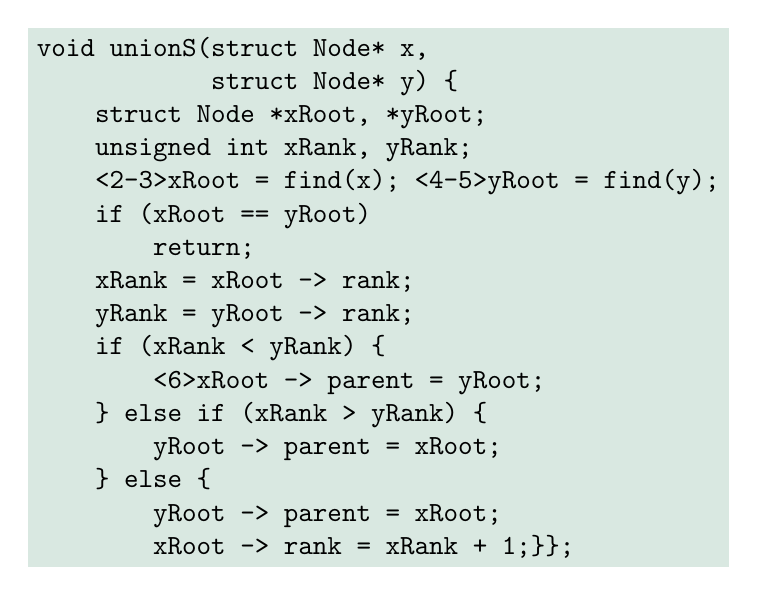
\begin{tikzpicture}
        \node [rectangle, fill=lightg] {
\begin{BVerbatim}[commandchars=\\\[\]]
\emphd[void] unionS(\emphd[struct] Node* x,
            \emphd[struct] Node* y) {
    \emphd[struct] Node *xRoot, *yRoot;
    unsigned int xRank, yRank;
    \emphr[2-3][xRoot = find(x)]; \emphr[4-5][yRoot = find(y)];
    \emphd[if] (xRoot == yRoot)
        \emphd[return];
    xRank = xRoot -> rank;
    yRank = yRoot -> rank;
    \emphd[if] (xRank < yRank) {
        \emphr[6][xRoot -> parent = yRoot];
    } \emphd[else if] (xRank > yRank) {
        yRoot -> parent = xRoot;
    } \emphd[else] {
        yRoot -> parent = xRoot;
        xRoot -> rank = xRank + 1;}};
\end{BVerbatim}
      };
      \end{tikzpicture}
    \column{.4\textwidth}
    \centering
    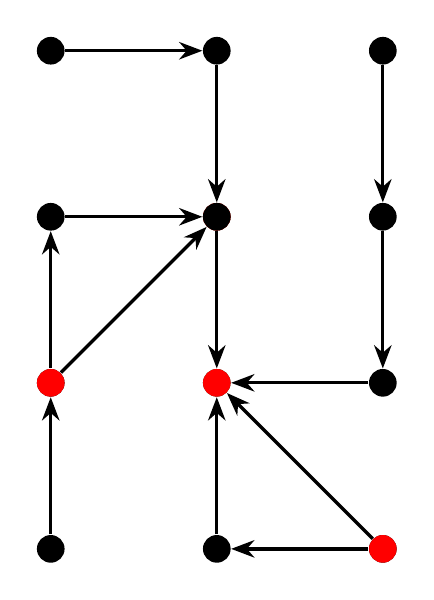
\begin{tikzpicture}[
        gn/.style={circle, inner sep=0pt, minimum size=10pt, fill=black},
        rn/.style={circle, inner sep=0pt, minimum size=10pt, fill=darkg},
        mn/.style={circle, inner sep=0pt, minimum size=10pt, fill=red},
        ->/.style={-Stealth, very thick}]
      \matrix[row sep=50, column sep=50]{
        \node[gn] (g1) {}; & \node[gn] (g2) {}; & \node[gn] (g3) {};\\
        \node[gn] (g4) {}; & \node<1-2>[rn] (g5) {}; \node<3-5>[mn] (g5) {};
        \node<6->[gn] (g5) {}; & \node[gn] (g6) {};\\
        \node<1,3->[gn] (g7) {}; \node<2>[mn] (g7) {}; & \node<1-4,6->[rn] (g8) {};
        \node<5>[mn] (g8) {}; & \node[gn] (g9) {}; \\
        \node[gn] (g10) {}; & \node[gn] (g11) {}; & \node<1-3,5->[gn] (g12) {};
        \node<4>[mn] (g12) {}; \\
      };
      \draw [->] (g10) to (g7);
      \draw<1-2> [->] (g7) to (g4);
      \draw<3-> [->] (g7) to (g5);
      \draw [->] (g4) to (g5);
      \draw [->] (g1) to (g2);
      \draw [->] (g2) to (g5);
      \draw [->] (g3) to (g6);
      \draw [->] (g6) to (g9);
      \draw [->] (g9) to (g8);
      \draw<1-4> [->] (g12) to (g11);
      \draw<5-> [->] (g12) to (g8);
      \draw [->] (g11) to (g8);
      \draw<6> [->] (g5) to (g8);
    \end{tikzpicture}
  \end{columns}
\end{frame}
}

\section{Outline}
\begin{frame}
  \begin{itemize}
  \item Motivation \hspace{1ex}\alert{\Large\checkmark}
  \item The Mathematical Graph Library
    \begin{itemize}
    \item Core Definitions
    \item Architecture
    \item Selection of Properties
    \end{itemize}
  \item The Spatial Representation of Graphs
    \begin{itemize}
    \item CompCert and VST
    \item Hoare Logic and Separation Logic
    \item Spatial Representation of Graphs
    \item Localize Rule
    \end{itemize}
  \item Verification of the Find function
    \begin{itemize}
    \item Specification
    \item Proof Skeleton
    \item Modularity
    \end{itemize}
  \item A Generational Garbage Collector
  \end{itemize}
\end{frame}

\section{The Mathematical Graph Library}
\subsection{Core Definitions}

\begin{frame}{Graph Library: A General Definition of Graph}
\small
    \begin{columns}[c]
      \column{.4\textwidth}
      \centering
      \colorbox{lightg}{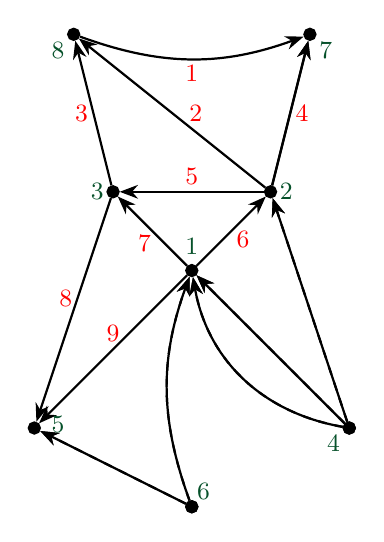
\begin{tikzpicture}
          [vad/.style={circle, fill=black, draw=black, thick,
              inner sep=0pt, minimum size=4pt},
            inv/.style={circle, draw=black, thick, inner sep=0pt, minimum size=4pt},
            ->/.style={thick, arrows={-Stealth}}]
          \node[vad] (n1) at (0, 0) {};
          \node[vad] (n2) at (1, 1) {};
          \node[vad] (n3) at (-1, 1) {};
          \node<1-4>[vad] (n4) at (2, -2) {};
          \node<5->[inv] (n4) at (2, -2) {};
          \node[vad] (n5) at (-2, -2) {};
          \node<1-4>[vad] (n6) at (0, -3) {};
          \node<5->[inv] (n6) at (0, -3) {};
          \node[vad] (n7) at (1.5, 3) {};
          \node[vad] (n8) at (-1.5, 3) {};
          \draw[->] (n1) to (n2);
          \draw[->] (n1) to (n3);
          \draw[->] (n3) to (n5);
          \draw[->] (n2) to (n3);
          \draw[->] (n2) to (n7);
          \draw[->] (n2) to (n7);
          \draw[->] (n2) to (n8);
          \draw[->] (n3) to (n8);
          \draw<1-4>[->] (n4) to (n1);
          \draw<5->[->, dashed] (n4) to (n1);
          \draw[->] (n1) to (n5);
          \draw<1-4>[->] (n4) to (n2);
          \draw<5->[->, dashed] (n4) to (n2);
          \draw<1-4>[->] (n6) to [bend left=20] (n1);
          \draw<5->[->, dashed] (n6) to [bend left=20] (n1);
          \draw<1-4>[->] (n6) to (n5);
          \draw<5->[->, dashed] (n6) to (n5);
          \draw[->] (n8) to [bend right=20] (n7);
          \uncover<3-4>{\draw[->] (n4) to [bend left=35] (n1);}
          \draw<5->[->, dashed] (n4) to [bend left=35] (n1);
          \node<8-> [darkg] at (0, 0.3) {\small $1$};
          \node<8-> [darkg] at (1.2, 1) {\small $2$};
          \node<8-> [darkg] at (-1.2, 1) {\small $3$};
          \node<8-> [darkg] at (1.8, -2.2) {\small $4$};
          \node<8-> [darkg] at (-1.7, -1.95) {\small $5$};
          \node<8-> [darkg] at (0.15, -2.8) {\small $6$};
          \node<8-> [darkg] at (1.7, 2.8) {\small $7$};
          \node<8-> [darkg] at (-1.7, 2.8) {\small $8$};
          \node<8-> [red] at (0, 2.5) {\small $1$};
          \node<8-> [red] at (0.05, 2) {\small $2$};
          \node<8-> [red] at (-1.4, 2) {\small $3$};
          \node<8-> [red] at (1.4, 2) {\small $4$};
          \node<8-> [red] at (0, 1.2) {\small $5$};
          \node<8-> [red] at (0.65, 0.4) {\small $6$};
          \node<8-> [red] at (-0.6, 0.35) {\small $7$};
          \node<8-> [red] at (-1.6, -0.35) {\small $8$};
          \node<8-> [red] at (-1, -0.8) {\small $9$};
        \end{tikzpicture}}
      \column{.6\textwidth}
      \only<1-6>{
        A general definition of graph should have
        \uncover<2->{\begin{itemize}
          \item Vertices
          \item \only<2,3>{Pairs of vertices as Edges}
            \only<4->{Edges, sources and destinations}
          \item<6-> Validity of vertices and edges
      \end{itemize}}}
      \only<7->{
        \begin{gather*}
          \begin{aligned}
            \mathrm{PreGraph}\defeq\{& V,\, E,\, \mathtt{vvalid},\,\mathtt{evalid},\\
            & \mathtt{src},\, \mathtt{dst}\}
          \end{aligned}\\
          \uncover<9->{\begin{aligned}
            \mathrm{LabeledGraph}\defeq\{&\mathrm{PreGraph},\,L_V,\,L_E,\,L_G,\\
            & \mathtt{vlabel},\,\mathtt{elabel},\,\mathtt{glabel}\}
          \end{aligned}\\}
          \uncover<10->{\mathrm{GeneralGraph}\defeq\{\mathrm{LabeledGraph},\,
            \mathtt{sound\_gg}\}\\}
          \uncover<11->{\text{For Example: Acyclic}}
        \end{gather*}
      }
    \end{columns}
\end{frame}

\begin{frame}{Graph Library: Definition of Path}
      \begin{columns}[c]
        \column{.4\textwidth}
        \centering
        \colorbox{lightg}{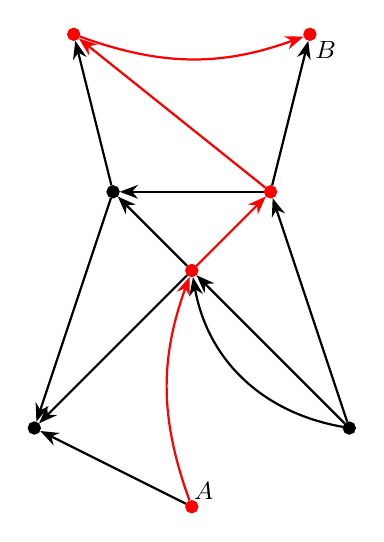
\begin{tikzpicture}
            [vad/.style={circle, fill=black, draw=black, thick,
                inner sep=0pt, minimum size=4pt},
              mrk/.style={circle, fill=red, draw=red, thick,
                inner sep=0pt, minimum size=4pt},
              ->/.style={thick, arrows={-Stealth}}]
            \node[mrk] (n1) at (0, 0) {};
            \node[mrk] (n2) at (1, 1) {};
            \node[vad] (n3) at (-1, 1) {};
            \node[vad] (n4) at (2, -2) {};
            \node[vad] (n5) at (-2, -2) {};
            \node[mrk] (n6) at (0, -3) {};
            \node[mrk] (n7) at (1.5, 3) {};
            \node[mrk] (n8) at (-1.5, 3) {};
            \node at (0.15, -2.8) {\small $A$};
            \node at (1.7, 2.8) {\small $B$};
            \draw[->, red] (n1) to (n2);
            \draw[->] (n3) to (n5);
            \draw[->] (n2) to (n3);
            \draw[->] (n2) to (n7);
            \draw[->, red] (n2) to (n8);
            \draw[->] (n1) to (n5);
            \draw[->, red] (n6) to [bend left=20] (n1);
            \draw[->] (n6) to (n5);
            \draw[->] (n4) to [bend left=35] (n1);
            \draw[->, red] (n8) to [bend right=20] (n7);
            \draw[->] (n3) to (n8);
            \draw[->] (n4) to (n1);
            \draw[->] (n4) to (n2);
            \draw[->] (n1) to (n3);
        \end{tikzpicture}}
        \column{.6\textwidth}
        \begin{itemize}
        \item<1-> Path is used in defining reachability.
        \item<2-> A path is a sequence of edges which connect a sequence of vertices.
        \end{itemize}
        \vspace{0.3cm}
        \uncover<3->{
          \begin{equation*}
            \textcolor<4->
                {gray}
                {\mathrm{Path}\,\defeq\, [v_0, e_0, v_1, e_1,
                  \dots, v_{k-1}, e_{k-1}, v_k]}
          \end{equation*}
          \uncover<4->{
            \begin{equation*}
              \textcolor<5->{gray}{\mathrm{Path}\,\defeq\, [e_0, e_1, \dots, e_k]}
          \end{equation*}}
          \uncover<5->{
            \begin{equation*}
              \mathrm{Path}\,\defeq\, (v_0, [e_0, e_1, \dots, e_k])
          \end{equation*}}
        }
      \end{columns}
\end{frame}

\begin{frame}{Other Derived Definitions: A Peek}
\small
  \begin{gather*}
    \begin{split}
    \mathtt{s\_evalid}(\gamma, e)\,\defeq\,& \mathtt{evalid}(\gamma, e)\wedge\null\\
    & \mathtt{vvalid}(\gamma, \mathtt{src}(\gamma,e))\wedge
    \mathtt{vvalid}(\gamma, \mathtt{dst}(\gamma,e))
    \end{split}\\
    \uncover<2->{
      \begin{split}
        \mathtt{valid\_path}\big(\gamma, (v,[])\big)\,\defeq\,&
        \mathtt{vvalid}(\gamma, v)\\
        \mathtt{valid\_path}\big(\gamma, (v,[e_1,e_2,\dots,e_n])\big)\,\defeq\,&
        v=\mathtt{src}(\gamma,e_1)\wedge
    \mathtt{s\_evalid}(\gamma,e_1)\wedge\null\\
    &\mathtt{dst}(\gamma,e_1)=\mathtt{src}(\gamma,e_2)\wedge\null\\
    &\mathtt{s\_evalid}(\gamma, e_2)\wedge\dots\\
      \end{split}\\
    }
    \uncover<3->{
      \begin{split}
      \mathtt{end}\big(\gamma, (v, [])\big)\,\defeq\,& v\\
      \mathtt{end}\big(\gamma, (v,[e_1,e_2,\dots,e_n])\big)\,\defeq\,&
      \mathtt{dst}(\gamma, e_n)\\
      \gamma \vDash s \overset{p}{\leadsto} t \;\defeq\; &
        \mathtt{valid\_path}(\gamma, p)\wedge
        \mathtt{fst}(p)=s \wedge \mathtt{end}(\gamma,p)=t\\
        \gamma \vDash s \leadsto t \;\defeq\; &
        \exists p \; \text{s.t.}\; \gamma \vDash s \overset{p}{\leadsto} t
      \end{split}
    }
  \end{gather*}
\end{frame}

\subsection{Architecture}
\begin{frame}{Architecture}
  \centering
  \colorbox{lightg}{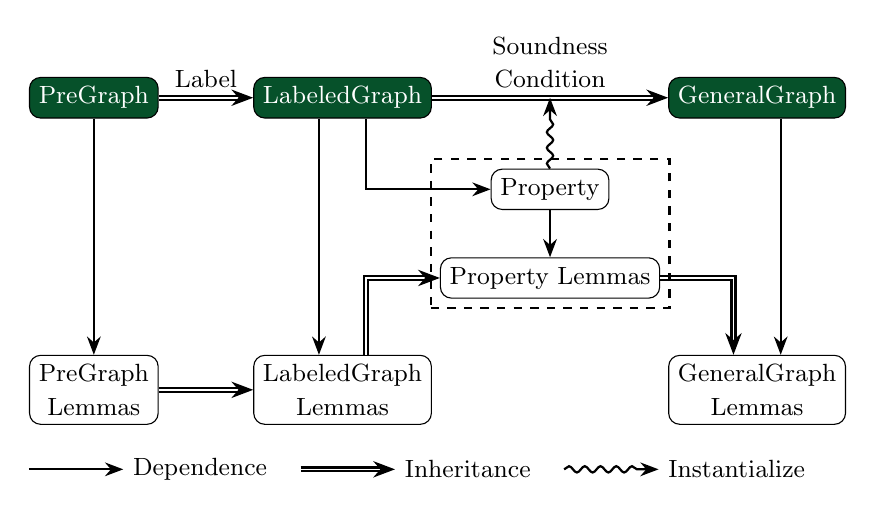
\begin{tikzpicture}
[->/.style={thick,arrows={-Stealth}},
-->/.style={thick,arrows={-Stealth}, decorate, decoration={snake, amplitude=.4mm,segment length=2mm,post length=2mm}},
   realG/.style={shape=rectangle, rounded corners=4pt, draw, fill=darkg},
   propG/.style={shape=rectangle, rounded corners=4pt, draw},
   x=1.5cm, y=1.5cm]
\node[realG] (PG) at (0, 0) {\small\color{white} PreGraph};
\node[realG] (LG) [right=0.8 of PG] {\small\color{white} LabeledGraph};
\node[realG] (GG) [right=2 of LG] {\small\color{white} GeneralGraph};
\draw [double, ->] (PG) -- (LG) node [pos=0.5, above] {\small Label} ;
\draw [double, ->] (LG) -- (GG) node (SC) [pos=0.5, above, align=center]
{\small Soundness \\ \small Condition};
\node[propG] (Prop) [below=0.6 of SC] {\small Property};
\node[propG] (PropL) [below=0.4 of Prop] {\small Property Lemmas};
\node[propG] (PGL) [below=2 of PG, align=center] {\small PreGraph \\\small Lemmas};
\node[propG] (LGL) [below=2 of LG, align=center] {\small LabeledGraph \\\small Lemmas};
\node[propG] (GGL) [below=2 of GG, align=center] {\small GeneralGraph \\\small Lemmas};
\draw [double, ->] (PGL) to (LGL);
%% \draw [double, ->] (LGL) to (GGL);
\draw [->] (PG) to (PGL);
\draw [->] (Prop) to (PropL);
\draw [-->] (Prop) to (SC);
\coordinate [left=0.2 of LG.south] (LGs1);
\coordinate [left=0.2 of LGL.north] (LGLn1);
\draw [->] (LGs1) to (LGLn1);
\coordinate [right=0.2 of LG.south] (LGs2);
\coordinate [right=0.2 of LGL.north] (LGLn2);
\draw [->] (LGs2) |- (Prop);
\draw [double, ->] (LGLn2) |- (PropL);
\coordinate [right=0.2 of GG.south] (GGs);
\coordinate [left=0.2 of GGL.north] (GGLn1);
\coordinate [right=0.2 of GGL.north] (GGLn2);
\draw [double, ->] (PropL) -| (GGLn1);
\draw [->] (GGs) to (GGLn2);
\node [draw, thick, rectangle, dashed, fit=(Prop) (PropL)] {};
\node (legend1) [below right=0.2 and -0.3 of PGL] {\small Dependence};
\coordinate[left=0.8 of legend1]  (l1);
\draw [->] (l1) to (legend1);
\node (legend2) [right=1 of legend1] {\small Inheritance};
\coordinate[left=0.8 of legend2]  (l2);
\draw [double, ->] (l2) to (legend2);
\node (legend3) [right=1 of legend2] {\small Instantialize};
\coordinate[left=0.8 of legend3]  (l3);
\draw [-->] (l3) to (legend3);
\end{tikzpicture}
}
\end{frame}

\subsection{Properties}
\begin{frame}[fragile]{Various Properties: MathGraph, LstGraph and FiniteGraph}
\small
  \begin{columns}[c]
    \column{.4\textwidth}
    \centering
    \colorbox{lightg}{
      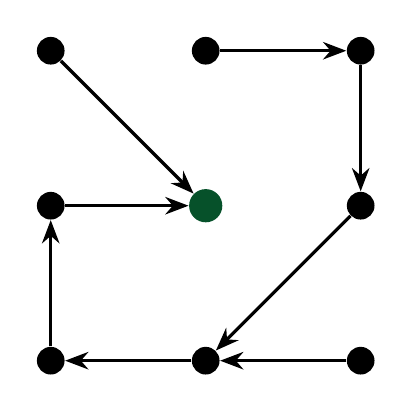
\begin{tikzpicture}[
          gn/.style={circle, inner sep=0pt, minimum size=10pt, fill=black},
          rn/.style={circle, inner sep=0pt, minimum size=12pt, fill=darkg},
          ->/.style={-Stealth, very thick}]
        \matrix[row sep=45, column sep=45, ampersand replacement=\&]{
          \node[gn] (g1) {}; \& \node[gn] (g2) {}; \& \node[gn] (g3) {};\\
          \node[gn] (g4) {}; \& \node[rn] (g5) {}; \& \node[gn] (g6) {};\\
          \node[gn] (g7) {}; \& \node[gn] (g8) {}; \& \node[gn] (g9) {}; \\
        };
        \draw [->] (g1) to (g5);
        \draw [->] (g2) to (g3);
        \draw [->] (g3) to (g6);
        \draw [->] (g6) to (g8);
        \draw [->] (g9) to (g8);
        \draw [->] (g8) to (g7);
        \draw [->] (g7) to (g4);
        \draw [->] (g4) to (g5);
      \end{tikzpicture}}
    \column{.6\textwidth}
    \begin{minipage}[c][\frametextheight][c]{\linewidth}
      \only<2>{
        \begin{align*}
        \mathrm{MathGraph}(\gamma)\,\defeq\, & \Big\{\\
          \mathtt{null}:\; & V\\
          \mathtt{weak\_valid}(v)\,\defeq\, & v = \mathtt{null} \vee
          \mathtt{vvalid}(\gamma, v)\\
          \mathtt{valid\_graph}:\;& \forall e\,.\,\mathtt{evalid}(\gamma, e)
          \Rightarrow\\
          & \mathtt{vvalid}\Big(\gamma, \mathtt{src}(\gamma, e)\Big)\wedge\null\\
          & \mathtt{weak\_valid}\Big(\mathtt{dst}(\gamma, e)\Big)\\
          \mathtt{valid\_not\_null}:\;& \forall v\,.\,\mathtt{vvalid}(\gamma, v)
          \Rightarrow \\ & v \neq \mathtt{null} \Big\}
      \end{align*}}
      \only<3>{
      \begin{align*}
        \mathrm{LstGraph}(\gamma)\,\defeq\, & \Big\{\\
        \mathtt{out}:\; & V \rightarrow E\\
        \mathtt{only\_one\_edge}:\; & \forall v,\,e\,.\,
         \mathtt{vvalid}(\gamma, v) \Rightarrow \\
         & \Big(\mathtt{src}(\gamma, e) =v \wedge \null\\
         & \mathtt{evalid}(\gamma, e)\Big) \Leftrightarrow\\
         & e = \mathtt{out}(v)\\
         \mathtt{acyclic\_path}:\; & \forall v,\,p\,.\,
         \gamma \vDash v \overset{p}{\leadsto} v \Rightarrow\\
         & p = (v,[])\Big\}
      \end{align*}}
      \only<4>{
      \begin{align*}
        \mathrm{FiniteGraph}(\gamma)\,\defeq\, & \Big\{\\
        \mathtt{finite\_v}:\;&\exists\, S_v,\, M_v\;\text{s.t.}\;\lvert S_v\rvert
        \leq M_v \wedge\null\\
        & \forall v\,.\, \mathtt{vvalid}(\gamma,v)\Rightarrow v\,\in\,S_v\\
        \mathtt{finite\_e}:\;&\exists\, S_e,\, M_e\;\text{s.t.}\;\lvert S_e\rvert
        \leq M_e \wedge \null\\
        &\forall e\,.\, \mathtt{evalid}(\gamma,e)\Rightarrow e\,\in\,S_e
         \Big\}
      \end{align*}}
    \end{minipage}
  \end{columns}
\end{frame}

\begin{frame}{Various Properties}
  \newcommand*{\myRadius}{1.7cm}
  \centering
  \begin{tikzpicture}[
      elp/.style={ellipse, x radius=2*\myRadius, y radius=\myRadius,
        minimum width=4*\myRadius, minimum height=2*\myRadius}]
    \node<1>[fill=darkg, elp, rotate=50] (elp1) at (1.6, 0) {};
    \uncover<2->{\node (MathGraph) at (4.5, 3) {MathGraph};}
    \node<2>[fill=darkg, elp, rotate=50] (elp1) at (0.3, 1) {};
    \uncover<3->{\node (LstGraph) at (3.2, 4) {LstGraph};}
    \node<3>[fill=darkg, elp, rotate=-50] (elp3) at (-0.3, 1) {};
    \uncover<4->{\node(FiniteGraph) at (-3.2, 4) {FiniteGraph};}
    \node<4>[fill=darkg, elp, rotate=-50] (elp3) at (-1.6, 0) {};
    \uncover<5>{\node(BiGraph) at (-4.5, 3) {BiGraph};}
    \node<-5>[draw, elp, rotate=50] (elp1) at (1.6, 0) {};
    \node<-5>[draw, elp, rotate=50] (elp2) at (0.3, 1) {};
    \node<-5>[draw, elp, rotate=-50] (elp3) at (-1.6, 0) {};
    \node<-5>[draw, elp, rotate=-50] (elp4) at (-0.3, 1) {};
    \node<1> (MathGraph) at (1.6, 0) {\color{white} MathGraph};
    \node<2> (LstGraph) at (0.3, 1) {\color{white} LstGraph};
    \node<3> (FiniteGraph) at (-0.3, 1) {\color{white} FiniteGraph};
    \node<4> (BiGraph) at (-1.6, 0) {\color{white} BiGraph};
  \end{tikzpicture}
\end{frame}

\section{Outline}
\begin{frame}
  \begin{itemize}
  \item Motivation \hspace{1ex}\alert{\Large\checkmark}
  \item The Mathematical Graph Library \hspace{1ex}\alert{\Large\checkmark}
    \begin{itemize}
    \item Core Definitions \hspace{1ex}\alert{\Large\checkmark}
    \item Architecture \hspace{1ex}\alert{\Large\checkmark}
    \item Selection of Properties \hspace{1ex}\alert{\Large\checkmark}
    \end{itemize}
  \item The Spatial Representation of Graphs
    \begin{itemize}
    \item CompCert and VST
    \item Hoare Logic and Separation Logic
    \item Spatial Representation of Graphs
    \item Localize Rule
    \end{itemize}
  \item Verification of the Find function
    \begin{itemize}
    \item Specification
    \item Proof Skeleton
    \item Modularity
    \end{itemize}
  \item A Generational Garbage Collector
  \end{itemize}
\end{frame}

\section{The Spatial Inference of Graph}
\subsection{CompCert and VST}
\begin{frame}{CompCert and VST}
  \credit{\footnotesize (Leroy et al.\ , Appel et al.)}
  \begin{columns}[c]
    \column{.5\textwidth}
    \centering
    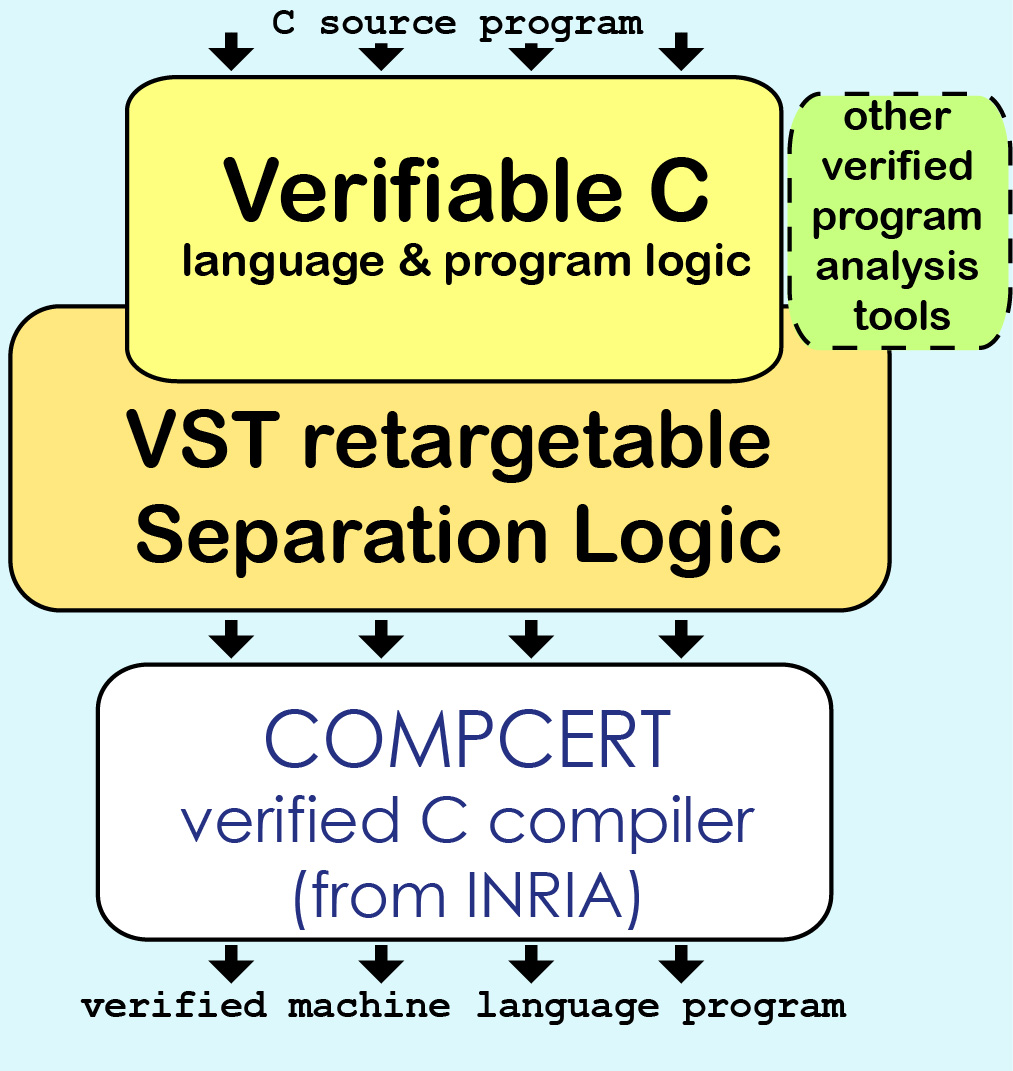
\includegraphics[width=\textwidth,keepaspectratio]{VST-diagram.jpg}
    \column{.5\textwidth}
    \begin{itemize}
    \item CompCert
      \begin{itemize}
      \item<2-> C $\rightarrow$ Coq (Clight) $\rightarrow$ Machine
      \item<3-> Full-Scale C Specification
      \end{itemize}
    \item<4-> Verified Software Toolchain
      \begin{itemize}
      \item<5-> Separation Hoare Logic
      \item<6-> Verifiable C
      \item<7-> Interactive Symbolic Execution
      \end{itemize}
    \end{itemize}
  \end{columns}
\end{frame}

\subsection{Hoare Logic and Separation Logic}
\begin{frame}{Recap: Hoare Logic}
  \credit{\footnotesize (C.\ A.\ R.\ Hoare)}
  \begin{equation*}
    \{P\}\,C\,\{Q\}
  \end{equation*}
\end{frame}

\newcommand*{\varwidth}[1]{{\vrule height 0pt depth 0cm width #1}}

\begin{frame}{Recap: Separation Logic}
  \credit{\footnotesize (Reynolds et al.)}
  \begin{center}
    \uncover<2->{
    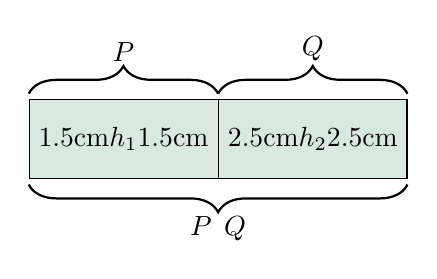
\begin{tikzpicture}
      \node [rectangle split, rectangle split horizontal, rectangle split parts=2,
        draw, minimum height=1cm, rectangle split part fill={lightg, lightg}]
      (heap) {\varwidth{1.5cm}$h_1$\varwidth{1.5cm}
        \nodepart{second}\varwidth{2.5cm}$h_2$\varwidth{2.5cm}};
      \draw[thick, decoration={brace, amplitude=10pt, raise=2pt},decorate]
      (heap.north west) -- node[above=10pt] {$P$} (heap.one split north);
      \draw[thick, decoration={brace, amplitude=10pt, raise=2pt},decorate]
      (heap.one split north) -- node[above=10pt] {$Q$} (heap.north east);
      \draw[thick, decoration={brace, mirror, amplitude=10pt, raise=2pt},decorate]
      (heap.south west) -- node[below=10pt] {$P \scon Q $} (heap.south east);
    \end{tikzpicture}}
  \end{center}
  \begin{equation*}
    \uncover<2->{h\models} P \scon Q\uncover<2->{\defeq \exists\, h_1, h_2\,\text{s.t.}\, h_1\oplus h_2 = h \wedge h_1\models P \wedge h_2\models Q}
  \end{equation*}
\end{frame}

\begin{frame}{Recap: Separation Logic}
  \credit{\footnotesize (Reynolds et al.)}
  \begin{center}
    \uncover<2->{
    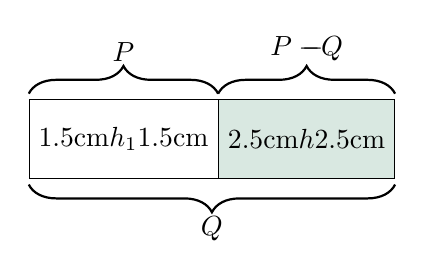
\begin{tikzpicture}
      \node [rectangle split, rectangle split horizontal, rectangle split parts=2,
        draw, minimum height=1cm, rectangle split part fill={white, lightg}]
      (heap) {\varwidth{1.5cm}$h_1$\varwidth{1.5cm}
        \nodepart{second}\varwidth{2.5cm}$h$\varwidth{2.5cm}};
      \draw[thick, decoration={brace, amplitude=10pt, raise=2pt},decorate]
      (heap.north west) -- node[above=10pt] {$P$} (heap.one split north);
      \draw[thick, decoration={brace, amplitude=10pt, raise=2pt},decorate]
      (heap.one split north) -- node[above=10pt] {$P \wand Q$} (heap.north east);
      \draw[thick, decoration={brace, mirror, amplitude=10pt, raise=2pt},decorate]
      (heap.south west) -- node[below=10pt] {$Q$} (heap.south east);
    \end{tikzpicture}}
  \end{center}
  \begin{equation*}
    \uncover<2->{h \models}P \wand Q\uncover<2->{\defeq \forall h_1, h_2\,.\,
      h_1\oplus h = h_2 \Rightarrow h_1 \models P \Rightarrow h_2 \models Q}
  \end{equation*}
\end{frame}

\begin{frame}{Recap: Separation Logic}
  \credit{\footnotesize (Reynolds et al.)}
  \begin{equation*}
    \only<1>{\forall P, Q\,.\, P \scon (P \wand Q) \vdash Q}
    \only<2>{\mathtt{emp}}
    \only<3>{a \mapsto v}
    \only<4>{\frac{\{P\}\,C\,\{Q\}}{\{P \scon F\}\,C\,\{Q \scon F \}}
    (\mathtt{mod}(C)\cap\mathtt{fv}(F)=\emptyset)}
  \end{equation*}
\end{frame}

\subsection{Spatial Representation of Graphs}
\begin{frame}[fragile]{Spatial Representation of Graphs}
    \begin{columns}[c]
    \column{.4\textwidth}
    \centering
    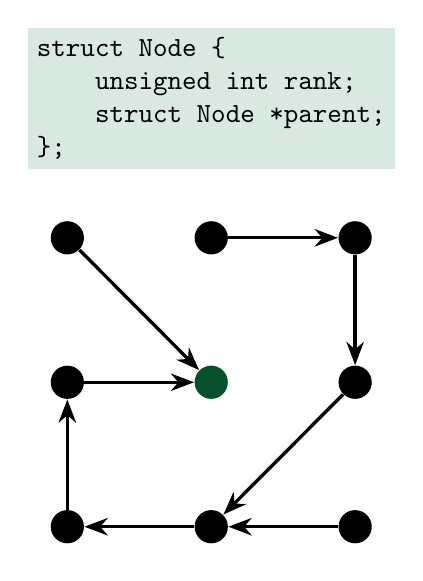
\begin{tikzpicture}[
        gn/.style={circle, inner sep=0pt, minimum size=12pt, fill=black},
        rn/.style={circle, inner sep=0pt, minimum size=12pt, fill=darkg},
        ->/.style={-Stealth, very thick}]
      \node [rectangle, fill=lightg] (struct) {
\begin{BVerbatim}[commandchars=\\\[\]]
\emphd[struct] Node {
    unsigned int rank;
    \emphd[struct] Node *parent;
};
\end{BVerbatim}
      };
      \node[matrix, row sep=40, column sep=40] (graph) [below=15pt of struct] {
        \node[gn] (g1) {}; & \node[gn] (g2) {}; & \node[gn] (g3) {};\\
        \node[gn] (g4) {}; & \node[rn] (g5) {}; & \node[gn] (g6) {};\\
        \node[gn] (g7) {}; & \node[gn] (g8) {}; & \node[gn] (g9) {}; \\
      };
      \draw [->] (g1) to (g5);
      \draw [->] (g2) to (g3);
      \draw [->] (g3) to (g6);
      \draw [->] (g6) to (g8);
      \draw [->] (g9) to (g8);
      \draw [->] (g8) to (g7);
      \draw [->] (g7) to (g4);
      \draw [->] (g4) to (g5);
    \end{tikzpicture}
    \column{.6\textwidth}
    \begin{center}\uncover<2->{
      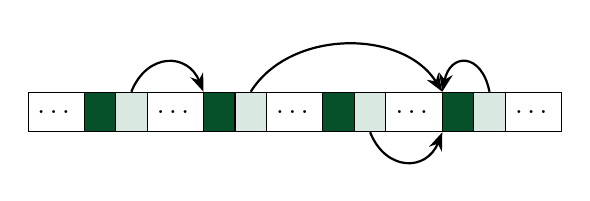
\begin{tikzpicture}[->/.style={-Stealth, thick}]
        \node [rectangle split, rectangle split horizontal, rectangle split parts=13,
          draw, minimum height=0.5cm, rectangle split part fill={white, darkg, lightg,
            white, darkg, lightg, white, darkg, lightg, white, darkg, lightg, white}]
        (heap) {\ldots\nodepart{four}\ldots\nodepart{seven}\ldots\nodepart{ten}\ldots
          \nodepart{thirteen}\ldots};
        \draw[->] (heap.three north)..controls +(0.2, 0.5) and +(-0.2, 0.5)..
        (heap.four split north);
        \draw[->] (heap.six north)..controls +(0.5, 0.8) and +(-0.5, 0.8)..
        (heap.ten split north);
        \draw[->] (heap.nine south)..controls +(0.2, -0.5) and +(-0.2, -0.5)..
        (heap.ten split south);
        \draw[->] (heap.twelve north)..controls +(-0.1, 0.5) and +(0.1, 0.5)..
        (heap.ten split north);
      \end{tikzpicture}}
    \end{center}
  \begin{gather*}
    \uncover<3->{\mathtt{graph\_rep}(\gamma)\,\defeq\,
      \underset{\mathtt{vvalid}(\gamma, v)}{\bigstar}\mathtt{v\_rep}(\gamma, v)\\}
    \uncover<4->{\underset{\{v_1, v_2, \dots, v_n\}}{\bigstar} P \,\defeq \,P(v_1)
      \scon P(v_2)\scon \dots\scon P(v_n)\\}
    \uncover<5->{\mathtt{v\_rep}(\gamma, v)\,\defeq\, v \mapsto
      \mathtt{vlabel}(\gamma, v) \scon \null\\
      (v + 4) \mapsto \mathtt{prt}(\gamma, v)\\}
    \uncover<6->{\mathtt{prt}(\gamma, v)\,\defeq\,
      \begin{cases}
        \mathtt{dst}(\gamma, \mathtt{out}(v)) & \neq\mathtt{null}\\
        v & \text{otherwise}\\
      \end{cases}}
  \end{gather*}
    \end{columns}
\end{frame}

%% \begin{frame}{Other Spatial Representations}
%%   \begin{equation*}
%%     \mathtt{graph\_rep}(x, \gamma)\,\defeq\,
%%     \underset{\gamma \vDash x \leadsto v}{\bigstar}\mathtt{v\_rep}(\gamma, v)
%%   \end{equation*}
%%   \uncover<2->{
%%     \begin{equation*}
%%       \mathtt{graph\_rep}(x, \gamma)\,\Leftrightarrow\,
%%       \mathtt{v\_rep(\gamma, x)} \ocon \hspace{-2ex}\underset{v\,\in\,
%%         \mathtt{nb}(\gamma, x)}{\medocon}\hspace{-2ex}\mathtt{graph\_rep(\gamma, v)}
%%     \end{equation*}}
%%   \uncover<3->{
%%     \begin{align*}
%%       h \vDash P \ocon Q \;\defeq\;& \exists h_1, h_2, h_3 \;\text{s.t.}\;
%%       (h_1\oplus h_2\oplus h_3=h)\wedge \null \\
%%       & (h_1 \oplus h_2 \vDash P) \wedge (h_2 \oplus h_3 \vDash P)\\
%%       \underset{\{v_1, v_2, \dots, v_n\}}{\medocon} \hspace{-3ex} P \;\defeq\;&P(v_1)
%%       \ocon P(v_2)\ocon \dots\ocon P(v_n)
%%     \end{align*}}
%% \end{frame}

\subsection{Localize Rule}
\begin{frame}{\textsc{Ramify} Rule}
  \credit{\footnotesize (Hobor and Villard)}
  \begin{center}
    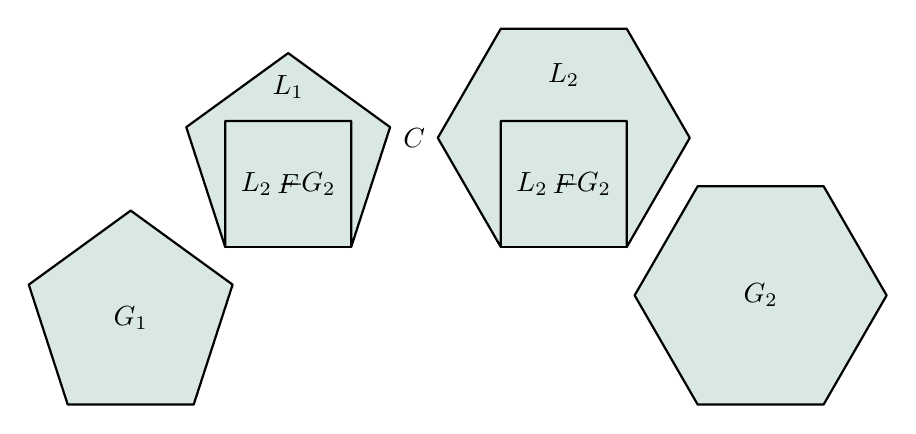
\begin{tikzpicture}[x=1.6cm, y=1.6cm, line join=round]
      \coordinate (six1) at (1, 0);
      \coordinate (six2) at (0.5, 0.866025);
      \coordinate (six3) at (-0.5, 0.866025);
      \coordinate (six4) at (-1, 0);
      \coordinate (six5) at (-0.5, -0.866025);
      \coordinate (six6) at (0.5, -0.866025);
      \coordinate (four1) at (0.5, 0.133975);
      \coordinate (four2) at (-0.5, 0.133975);
      \coordinate (five1) at (0.809017, 0.0850311);
      \coordinate (five2) at (0, 0.672816);
      \coordinate (five3) at (-0.809017, 0.0850311);
      \coordinate (mean four) at (0, -0.366025);
      \coordinate (mean five) at (0, -0.177834);
      \coordinate (mean six) at (0, 0);
      \coordinate (P) at (0, 0.403395);
      \coordinate (Q) at (0, 0.5);
      \draw[thick, fill=lightg] (five1) -- (five2) -- (five3) --
        (six5) -- (six6) -- cycle;
      \node at (mean five) {$G_1$};
      \draw[thick, fill=lightg] ([xshift=8cm]six1) -- ([xshift=8cm]six2) --
      ([xshift=8cm]six3) -- ([xshift=8cm]six4) -- ([xshift=8cm]six5) --
      ([xshift=8cm]six6) -- cycle;
      \node at ([xshift=8cm]mean six) {$G_2$};
      \uncover<3->{\draw[thick, fill=lightg] ([xshift=2cm,yshift=2cm]four1) --
        ([xshift=2cm,yshift=2cm]four2) -- ([xshift=2cm,yshift=2cm]six5) --
        ([xshift=2cm,yshift=2cm]six6) -- cycle;}
      \uncover<2->{\draw[thick, fill=lightg] ([xshift=2cm,yshift=2cm]six6) --
        ([xshift=2cm,yshift=2cm]five1) -- ([xshift=2cm,yshift=2cm]five2) --
        ([xshift=2cm,yshift=2cm]five3) -- ([xshift=2cm,yshift=2cm]six5) --
        ([xshift=2cm,yshift=2cm]four2) -- ([xshift=2cm,yshift=2cm]four1) -- cycle;
        \node at ([xshift=2cm,yshift=2cm]P) {$L_1$};}
      \uncover<3->{\draw[thick, fill=lightg] ([xshift=5.5cm,yshift=2cm]four1) --
        ([xshift=5.5cm,yshift=2cm]four2) -- ([xshift=5.5cm,yshift=2cm]six5) --
        ([xshift=5.5cm,yshift=2cm]six6) -- cycle;}
      \uncover<2->{\draw[thick, fill=lightg] ([xshift=5.5cm,yshift=2cm]six6) --
        ([xshift=5.5cm,yshift=2cm]six1) -- ([xshift=5.5cm,yshift=2cm]six2) --
        ([xshift=5.5cm,yshift=2cm]six3) -- ([xshift=5.5cm,yshift=2cm]six4) --
        ([xshift=5.5cm,yshift=2cm]six5) -- ([xshift=5.5cm,yshift=2cm]four2) --
        ([xshift=5.5cm,yshift=2cm]four1) -- cycle;
        \node at ([xshift=5.5cm,yshift=2cm]Q) {$L_2$};}
      \node<3,4> at ([xshift=2cm,yshift=2cm]mean four) {$F$};
      \node<3,4> at ([xshift=5.5cm,yshift=2cm]mean four) {$F$};
      \node<5-> at ([xshift=2cm,yshift=2cm]mean four) {$L_2 \wand G_2$};
      \node<5-> at ([xshift=5.5cm,yshift=2cm]mean four) {$L_2 \wand G_2$};
      \node at ([xshift=3.6cm, yshift=2cm]mean six) {$C$};
    \end{tikzpicture}
  \end{center}
  \begin{gather*}
    \frac{\uncover<2->{\{L_1\}\,C\,\{L_2\}}\quad
      \uncover<6->{G_1 \vdash L_1 \scon (L_2 \wand G_2)}}
         {\{G_1\}\,C\,\{G_2\}}\;
         \uncover<6->{(\mathtt{mod}(C)\cap\mathtt{fv}(L_2 \wand G_2)=\emptyset)\\}
         \uncover<4,5>{\alert{\text{Hint: }\forall P, Q\,.\, P \scon (P \wand Q)
             \vdash Q}}
  \end{gather*}
\end{frame}

%}

\begin{frame}{\textsc{Localize} Rule}
  \begin{equation*}
    \frac{\{ L_1 \}\,C\,\{\uncover<2->{{\color{red}{\exists x \,.\,}}} L_2\} \qquad
      G_1 \vdash L_1 \scon R \qquad
      R \vdash 
      \uncover<2->{{\color{red}{\forall x \,.\,(}}}
      L_2 \wand G_2\uncover<2->{{\color{red}{)}}}}
         {\{ G_1 \} \,C\, \{\uncover<2->{{\color{red}{\exists x \,.\,}}} G_2 \}} \uncover<3->{~~(\dagger)}
  \end{equation*}
%  \vfill
%  \begin{equation*}
%    \frac{G_1 \vdash L_1 \scon F \quad F \vdash
%      \uncover<2->{{\color{red}{\forall x \,.\,(}}}L_2 \wand G_2
%      \uncover<2->{{\color{red}{)}}}}
%         {G_1 \vdash L_1 \scon \pguards{C}
%         \big( \uncover<2->{{\color{red}{\forall x \,.\,(}}}
%         L_2 \wand G_2\uncover<2->{{\color{red}{)}}}\big)}\;
%         F \textsc{ ignores } \langle C \rangle
%  \end{equation*}
  \vspace{0.5em}
  \begin{align*}
   \uncover<3->{(\dagger)~~\mathtt{mod}(C)\cap\mathtt{fv}(R)=\emptyset\\}
  \end{align*}
  \vfill
\hide{  }
\uncover<4->{Comparing to Ramify rule:
  \begin{gather*}
    \frac{{\{L_1\}\,C\,\{L_2\}}\quad
      {G_1 \vdash L_1 \scon (L_2 \wand G_2)}}
         {\{G_1\}\,C\,\{G_2\}}\; ~~ (\ddagger)
  \end{gather*}
%  \vspace{0.5em}
  \begin{align*}
  (\ddagger) ~~ \mathtt{mod}(C)\cap\mathtt{fv}(L_2 \wand G_2)=\emptyset
  \end{align*}
}
\end{frame}

\hide{
\begin{frame}{\textsc{Ramify-P} and \textsc{Ramify-PQ} Rule}
  \begin{equation*}
    \frac{\{ L_1 \}\,C\,\{\uncover<2->{{\color{red}{\exists x \,.\,}}} L_2\} \quad
      G_1 \vdash L_1 \scon \pguards{C}\big(
      \uncover<2->{{\color{red}{\forall x \,.\,(}}}
      L_2 \wand G_2\uncover<2->{{\color{red}{)}}}\big)}
         {\{ G_1 \} \,C\, \{\uncover<2->{{\color{red}{\exists x \,.\,}}} G_2 \}}
  \end{equation*}
  \vfill
  \begin{equation*}
    \frac{G_1 \vdash L_1 \scon F \quad F \vdash
      \uncover<2->{{\color{red}{\forall x \,.\,(}}}L_2 \wand G_2
      \uncover<2->{{\color{red}{)}}}}
         {G_1 \vdash L_1 \scon \pguards{C}
         \big( \uncover<2->{{\color{red}{\forall x \,.\,(}}}
         L_2 \wand G_2\uncover<2->{{\color{red}{)}}}\big)}\;
         F \textsc{ ignores } \langle C \rangle
  \end{equation*}
  \vfill
  \small
  \begin{align*}
    \sigma \vDash \pguards{C} P \;& \defeq\; \forall \sigma'\;.\;
    (\sigma \stackrel{\langle C \rangle}{\cong} \sigma') \Rightarrow
    (\sigma' \vDash P)\\
    \sigma \stackrel{S}{\cong} \sigma' \; &\defeq \; \sigma \text{ and } \sigma'
    \text{ coincide everywhere except } S\\
    P \textsc{ ignores } S \;& \defeq\; \forall \sigma, \sigma' \;.\;
    \sigma \stackrel{S}{\cong} \sigma' \Rightarrow (\sigma |= P) \Leftrightarrow
    (\sigma' |= P)
  \end{align*}
\end{frame}
}

\section{Outline}
\begin{frame}
  \begin{itemize}
  \item Motivation \hspace{1ex}\alert{\Large\checkmark}
  \item The Mathematical Graph Library \hspace{1ex}\alert{\Large\checkmark}
    \begin{itemize}
    \item Core Definitions \hspace{1ex}\alert{\Large\checkmark}
    \item Architecture \hspace{1ex}\alert{\Large\checkmark}
    \item Selection of Properties \hspace{1ex}\alert{\Large\checkmark}
    \end{itemize}
  \item The Spatial Representation of Graphs \hspace{1ex}\alert{\Large\checkmark}
    \begin{itemize}
    \item CompCert and VST \hspace{1ex}\alert{\Large\checkmark}
    \item Hoare Logic and Separation Logic \hspace{1ex}\alert{\Large\checkmark}
    \item Spatial Representation of Graphs \hspace{1ex}\alert{\Large\checkmark}
    \item Localize Rule \hspace{1ex}\alert{\Large\checkmark}
    \end{itemize}
  \item Verification of the Find function
    \begin{itemize}
    \item Specification
    \item Proof Skeleton
    \item Modularity
    \end{itemize}
  \item A Generational Garbage Collector
  \end{itemize}
\end{frame}

\section{Verification of the Find function}
\subsection{Specification}
\begin{frame}[fragile]{Union-Find Algorithm: Find}
  \begin{columns}[c]
    \column{.6\textwidth}
    \centering
   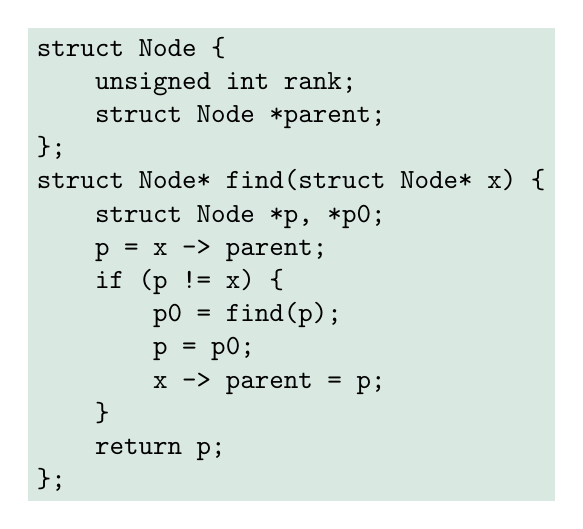
\begin{tikzpicture}
      \node [rectangle, fill=lightg] {
\begin{BVerbatim}[commandchars=\\\[\]]
\emphd[struct] Node {
    unsigned int rank;
    \emphd[struct] Node *parent;
};
\emphd[struct] Node* find(\emphd[struct] Node* x) {
    \emphd[struct] Node *p, *p0;
    p = x -> parent;
    \emphd[if] (p != x) {
        p0 = find(p);
        p = p0;
        x -> parent = p;
    }
    \emphd[return] p;
};
\end{BVerbatim}
      };
   \end{tikzpicture}
   \column{.4\textwidth}
   \centering
   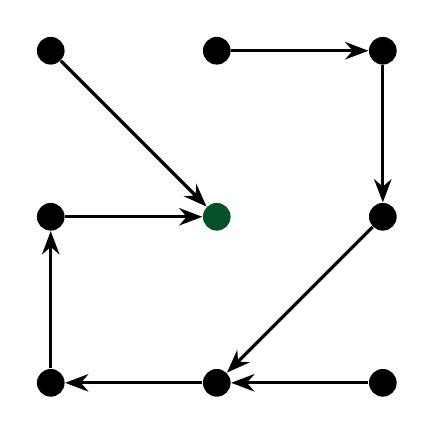
\begin{tikzpicture}[
       gn/.style={circle, inner sep=0pt, minimum size=10pt, fill=black},
       rn/.style={circle, inner sep=0pt, minimum size=10pt, fill=darkg},
       ->/.style={-Stealth, very thick}]
     \matrix[row sep=50, column sep=50]{
       \node[gn] (g1) {}; & \node[gn] (g2) {}; & \node[gn] (g3) {};\\
       \node[gn] (g4) {}; & \node[rn] (g5) {}; & \node[gn] (g6) {};\\
       \node[gn] (g7) {}; & \node[gn] (g8) {}; & \node[gn] (g9) {}; \\
     };
     \draw [->] (g1) to (g5);
     \draw [->] (g2) to (g3);
     \draw [->] (g3) to (g6);
     \draw [->] (g6) to (g8);
     \draw [->] (g9) to (g8);
     \draw [->] (g8) to (g7);
     \draw [->] (g7) to (g4);
     \draw [->] (g4) to (g5);
   \end{tikzpicture}
  \end{columns}
\end{frame}

\begin{frame}{The Specification of Find}
  \centering
  \colorbox{lightg}{\parbox{.9\textwidth}{
      \begin{description}
      \item[{\bf PRE:}] $\mathtt{graph\_rep}(\gamma) \wedge \mathtt{vvalid}(\gamma, x)$
      \item[{\bf POST:}] $\exists \gamma', t\;\text{s.t.}\;\mathtt{graph\_rep}(\gamma')\wedge\mathtt{uf\_eq}(\gamma, \gamma') \wedge \mathtt{root}(\gamma', x, t)$
  \end{description}}}
  \pause
  \vskip10pt
  \colorbox{lightg}{\parbox{.9\textwidth}{
      \begin{align*}
        \mathtt{graph\_rep}(\gamma)\;\defeq\; &
        \underset{\mathtt{vvalid}(\gamma, v)}{\bigstar}\mathtt{v\_rep}(\gamma, v)\\
        \mathtt{root}(\gamma, x, t) \;\defeq\; &\gamma \vDash x \leadsto t \wedge
        \forall y.~ \gamma \vDash t \leadsto y \Rightarrow y = t\\
        \mathtt{uf\_eq}(\gamma_1, \gamma_2)\; \defeq\; &\big(\forall x.~
        \mathtt{vvalid}(\gamma_1, x)\Leftrightarrow \mathtt{vvalid}(\gamma_2,x)\big)
        \, \wedge\, \null\\
        & \forall x, r_1, r_2.~ \mathtt{root}(\gamma_1, x, r_1) \Rightarrow\\
        &\mathtt{root}(\gamma_2, x, r_2) \Rightarrow r_1 = r_2
      \end{align*}
    }}
\end{frame}

\subsection{Proof Skeleton}

\begin{frame}{Proof Skeleton of Find}
  \centering
  \begin{tikzpicture}[node distance=0.4mm]
    \node (line 0) {\color<3-10>{lightgray}{$\{\mathtt{graph\_rep}(\gamma) \wedge
      \mathtt{vvalid}(\gamma, \mathtt{x})\}$}};
    \node (line 1) [below = of line 0] {\color<3-10>{lightgray}
      {\Verb|p = x -> parent;|}};
    \onslide<2->{\node (line 2) [below = of line 1]
      {\color<5-10>{lightgray}{$\{\mathtt{graph\_rep}(\gamma) \wedge
      \mathtt{vvalid}(\gamma, \mathtt{x})\wedge
      \mathtt{p}=\mathtt{prt}(\gamma, \mathtt{x})\}$}};}
    \node (line 3) [below = of line 2] {\color<2,5-10>{lightgray}
      {\Verb|p0 = find(p);|}};
    \onslide<4->{\node (line 4) [below = of line 3] {\color<7,9,10>{lightgray}
        {$\{\mathtt{graph\_rep}
          (\gamma_1)\wedge\mathtt{uf\_eq}(\gamma, \gamma_1) \wedge
          \mathtt{root}(\gamma_1, \mathtt{p}, \mathtt{p0})\wedge
          \mathtt{p}=\mathtt{prt}(\gamma, \mathtt{x})\}$}};}
    \onslide<7->{\node (line 5) [below = of line 4] {\color<9,10>{lightgray}
        {$\uncover<8->{\alert{\searrow}} \{\mathtt{x}\mapsto
          \mathtt{vlabel}(\gamma_1, \mathtt{x}),
          \mathtt{prt}(\gamma_1, \mathtt{x})\}$}};}
      \node (line 6) [below = of line 5] {\color<2-4,9,10>{lightgray}
        {\Verb|x -> parent = p0|}};
      \onslide<7->{\node (line 7) [below = of line 6] {\color<9,10>{lightgray}
          {$\uncover<8->{\alert{\swarrow}}
          \{\mathtt{x}\mapsto \mathtt{vlabel}(\gamma_1, \mathtt{x}), \mathtt{p0}\}$}};}
      \onslide<6->{\node (line 8) [below = of line 7] {\color<7>{lightgray}
          {$\{\mathtt{graph\_rep}
          (\gamma_2)\wedge\gamma_2=\mathtt{redirect\_parent}(\gamma_1,\mathtt{x},
          \mathtt{p0}) \wedge\dots\}$}};}
      \onslide<10->{\node (line 9) [below = of line 8] {$\{\mathtt{graph\_rep}
          (\gamma_2)\wedge\mathtt{uf\_eq}(\gamma, \gamma_2) \wedge \mathtt{root}
          (\gamma_2, \mathtt{x}, \mathtt{p0})\}$};}
      \onslide<1-11>{\node (line 10) [below = of line 9]
        {\color<2,5-8>{lightgray}{$\{\exists \gamma'.~
         \mathtt{graph\_rep}(\gamma')\wedge\mathtt{uf\_eq}(\gamma,
            \gamma') \wedge \mathtt{root}(\gamma', \mathtt{x}, \mathtt{p0})\}$}};}
  \end{tikzpicture}
\end{frame}

\begin{frame}{Proof Obligation of Find}
  \centering
  \colorbox{lightg}{\parbox{.9\textwidth}{
  \begin{align*}
    \mathtt{graph\_rep}(\gamma_1) \vdash & \big(\mathtt{x}\mapsto
    \mathtt{vlabel}(\gamma_1, \mathtt{x}), \mathtt{prt}(\gamma_1, \mathtt{x})\big)
    \scon \null\\
    & \Big(\big(\mathtt{x}\mapsto \mathtt{vlabel}(\gamma_1, \mathtt{x}),
    \mathtt{p0}\big) \wand \null\\
    & \mathtt{graph\_rep}\big(\mathtt{redirect\_parent}(\gamma_1,\mathtt{x},
    \mathtt{p0})\big)\Big)
  \end{align*}}}
  \pause
  \vskip15pt
  \colorbox{lightg}{\parbox{.9\textwidth}{
  \begin{align*}
    & \mathtt{uf\_eq}(\gamma, \gamma_1) \Rightarrow \mathtt{root}(\gamma_1, \mathtt{p},
    \mathtt{p0}) \Rightarrow \mathtt{dst}\big(\gamma, \mathtt{out}(\mathtt{x})\big)=
    \mathtt{p}\\
    & \gamma_2=\mathtt{redirect\_parent}(\gamma_1,\mathtt{x},\mathtt{p0}) \Rightarrow\\
    & \mathtt{uf\_eq}(\gamma, \gamma_2) \wedge \mathtt{root}(\gamma_2, \mathtt{x},
    \mathtt{p0})
  \end{align*}}}
\end{frame}

\subsection{Modularity}

\begin{frame}[fragile]{Modularity: The Array Version of Find}
  \begin{columns}[c]
    \column{.7\textwidth}
    \centering
    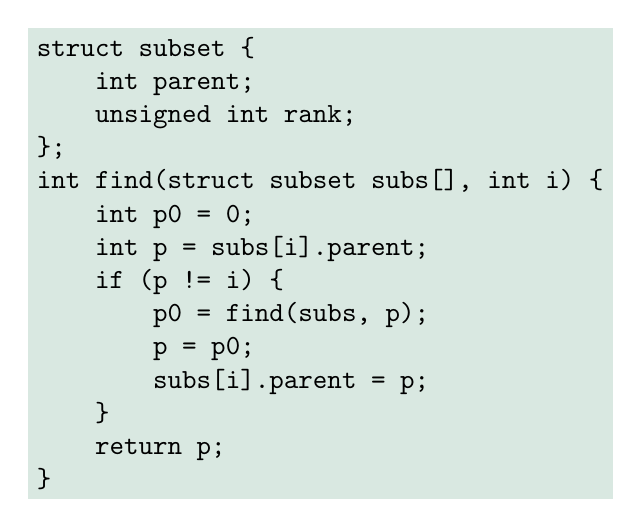
\begin{tikzpicture}
      \node [rectangle, fill=lightg] {
\begin{BVerbatim}[commandchars=\\\[\]]
\emphd[struct] subset {
    \emphd[int] parent;
    \emphd[unsigned] \emphd[int] rank;
};
\emphd[int] find(\emphd[struct] subset subs\bracket[], \emphd[int] i) {
    \emphd[int] p0 = 0;
    \emphd[int] p = subs\bracket[i].parent;
    \emphd[if] (p != i) {
        p0 = find(subs, p);
        p = p0;
        subs\bracket[i].parent = p;
    }
    \emphd[return] p;
}
\end{BVerbatim}
      };
    \end{tikzpicture}
    \column{.3\textwidth}
        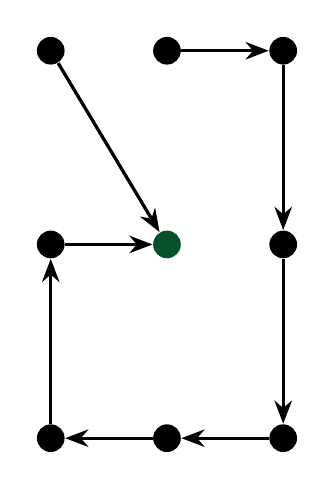
\begin{tikzpicture}[
            gn/.style={circle, inner sep=0pt, minimum size=10pt, fill=black},
            rn/.style={circle, inner sep=0pt, minimum size=10pt, fill=darkg},
            ->/.style={-Stealth, very thick}]
          \matrix[row sep=60, column sep=32]{
            \node[gn] (g1) {}; & \node[gn] (g2) {}; & \node[gn] (g3) {};\\
            \node[gn] (g4) {}; & \node[rn] (g5) {}; & \node[gn] (g6) {};\\
            \node[gn] (g7) {}; & \node[gn] (g8) {}; & \node[gn] (g9) {};\\
          };
          \draw [->] (g1) to (g5);
          \draw [->] (g2) to (g3);
          \draw [->] (g3) to (g6);
          \draw [->] (g6) to (g9);
          \draw [->] (g9) to (g8);
          \draw [->] (g8) to (g7);
          \draw [->] (g7) to (g4);
          \draw [->] (g4) to (g5);
        \end{tikzpicture}
  \end{columns}
\end{frame}

\begin{frame}{The same specification but a different representation}
  \centering
  \colorbox{lightg}{\parbox{.9\textwidth}{
      \begin{description}
      \item[{\bf PRE:}] $\mathtt{graph\_rep}(\gamma, s)
        \wedge \mathtt{vvalid}(\gamma, x)$
      \item[{\bf POST:}] $\exists \gamma', t\;\text{s.t.}\;\mathtt{graph\_rep}
        (\gamma', s)\wedge\mathtt{uf\_eq}(\gamma, \gamma') \wedge \mathtt{root}
        (\gamma', x, t)$
  \end{description}}}
  \pause
  \vskip20pt
  \colorbox{lightg}{\parbox{.9\textwidth}{
      \begin{align*}
        \mathtt{graph\_rep}(g, s) \quad \defeq \quad & \exists n.~
        \Big(\forall v.~ 0\leq v < n ~ \Leftrightarrow ~ \mathtt{vvalid}(\gamma, v)
        \wedge \null\\
      & \big(n \leq \mathrm{MaxInt}/8\big) \wedge \null \\
        & s \mapsto \mathtt{map}(\lambda v.~ \mathtt{v\_rep}(\gamma, v)) ~
               [0,1,2,\dots,n]\Big)
      \end{align*}
    }}
\end{frame}

\section{Outline}
\begin{frame}
  \begin{itemize}
  \item Motivation \hspace{1ex}\alert{\Large\checkmark}
  \item The Mathematical Graph Library \hspace{1ex}\alert{\Large\checkmark}
    \begin{itemize}
    \item Core Definitions \hspace{1ex}\alert{\Large\checkmark}
    \item Architecture \hspace{1ex}\alert{\Large\checkmark}
    \item Selection of Properties \hspace{1ex}\alert{\Large\checkmark}
    \end{itemize}
  \item The Spatial Representation of Graphs \hspace{1ex}\alert{\Large\checkmark}
    \begin{itemize}
    \item CompCert and VST \hspace{1ex}\alert{\Large\checkmark}
    \item Hoare Logic and Separation Logic \hspace{1ex}\alert{\Large\checkmark}
    \item Spatial Representation of Graphs \hspace{1ex}\alert{\Large\checkmark}
    \item Localize Rule \hspace{1ex}\alert{\Large\checkmark}
    \end{itemize}
  \item Verification of the Find function \hspace{1ex}\alert{\Large\checkmark}
    \begin{itemize}
    \item Specification \hspace{1ex}\alert{\Large\checkmark}
    \item Proof Skeleton \hspace{1ex}\alert{\Large\checkmark}
    \item Modularity \hspace{1ex}\alert{\Large\checkmark}
    \end{itemize}
  \item A Generational Garbage Collector
  \end{itemize}
\end{frame}

\section{Garbage Collector}

\begin{frame}{A Generational Garbage Collector}
  \begin{itemize}
  \item 12 generations; mutator allocates only into the first
  \item Functional mutator, so no backward pointers
  \pause
  \item Cheney's mark-and-copy collects generation to its successor
  \item Receiving generation may exceed fullness bound, \\
  triggering cascade of further pairwise collections
  \pause
  \item Most tasks are handled by a versatile \texttt{forward} function
  \end{itemize}
\end{frame}

\usetikzlibrary{positioning}


\begin{frame}[fragile]{Overview of \texttt{forward} (proposal)}
  \begin{center}
  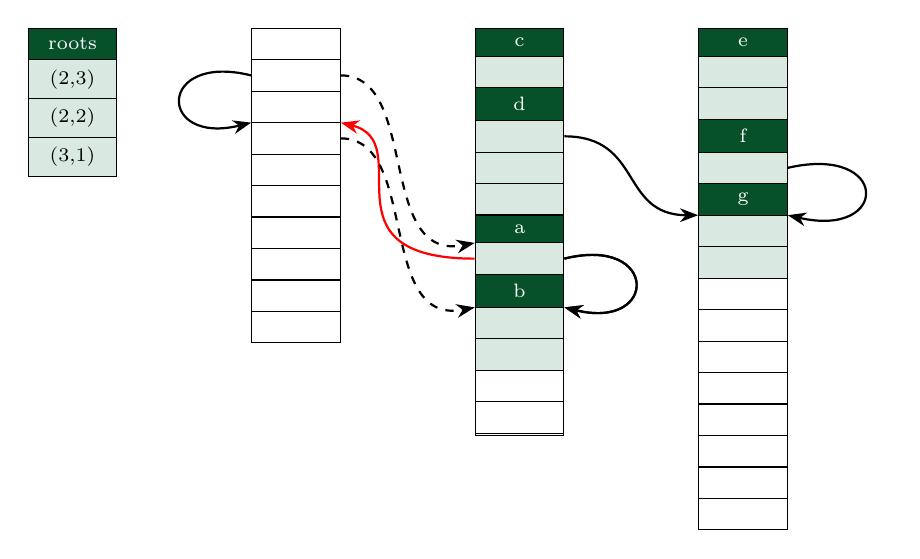
\begin{tikzpicture}[heap/.style={rectangle split, rectangle split parts=#1, draw,
        minimum width=32pt}, node distance=1.7cm, ->/.style={-Stealth, thick}]
    \node<1> [heap=10, rectangle split part fill={darkg, lightg,
        darkg, lightg, lightg, white}]
    (gen 0) {\color{white}{\scriptsize a}\nodepart{three}\color{white}{\scriptsize b}};
    \node<2> [heap=10, rectangle split part fill={red, lightg,
        darkg, lightg, lightg, white}]
    (gen 0) {\color{white}{\scriptsize a}\nodepart{three}\color{white}{\scriptsize b}};
    \node<3> [heap=10, rectangle split part fill={red, lightg,
        red, lightg, lightg, white}]
    (gen 0) {\color{white}{\scriptsize a}\nodepart{three}\color{white}{\scriptsize b}};
    \node<4> [heap=10, rectangle split part fill={red, lightg,
        red, lightg, lightg, white}]
    (gen 0) {\color{white}{\scriptsize a}\nodepart{three}\color{white}{\scriptsize b}};
    \node<5> [heap=10, rectangle split part fill={white}] (gen 0) {};

    \node<1>[heap=13, right = of gen 0.north east, anchor=north west,
      rectangle split part fill={darkg, lightg, darkg,
        lightg, lightg, lightg, white}] 
        (gen 1) {\color{white}{\scriptsize c}\nodepart{three}\color{white}{\scriptsize d}};
    \node<2>[heap=13, right = of gen 0.north east, anchor=north west,
      rectangle split part fill={darkg, lightg, darkg,
        lightg, lightg, lightg, darkg, lightg, white}] 
        (gen 1) {\color{white}{\scriptsize c}\nodepart{three}\color{white}{\scriptsize d}\nodepart{seven}\color{white}{\scriptsize a}};
    \node<3>[heap=13, right = of gen 0.north east, anchor=north west,
      rectangle split part fill={darkg, lightg, darkg,
        lightg, lightg, lightg, darkg, lightg, darkg, lightg, lightg,
        white}] (gen 1) 
        {\color{white}{\scriptsize c}\nodepart{three}\color{white}{\scriptsize d}\nodepart{seven}\color{white}{\scriptsize a}\nodepart{nine}\color{white}{\scriptsize b}};
    \node<4>[heap=13, right = of gen 0.north east, anchor=north west,
      rectangle split part fill={darkg, lightg, darkg,
        lightg, lightg, lightg, darkg, lightg, darkg, lightg, lightg,
        white}] 
        (gen 1) {\color{white}{\scriptsize c}\nodepart{three}\color{white}{\scriptsize d}\nodepart{seven}\color{white}{\scriptsize a}\nodepart{nine}\color{white}{\scriptsize b}};
    \node<5>[heap=13, right = of gen 0.north east, anchor=north west,
      rectangle split part fill={darkg, lightg, darkg,
        lightg, lightg, lightg, darkg, lightg, darkg, lightg, lightg,
        white}] 
        (gen 1) {\color{white}{\scriptsize c}\nodepart{three}\color{white}{\scriptsize d}\nodepart{seven}\color{white}{\scriptsize a}\nodepart{nine}\color{white}{\scriptsize b}};

    \node [heap=16, right = of gen 1.north east, anchor=north west,
      rectangle split part fill={darkg, lightg, lightg, darkg,
        lightg, darkg, lightg, lightg, white}]
    (gen 2) {\color{white}{\scriptsize e}\nodepart{four}\color{white}{\scriptsize f}\nodepart{six}\color{white}{\scriptsize g}};

    \node<1> [heap=4, left = of gen 0.north west, anchor=north east,
      rectangle split part fill={darkg, lightg, lightg, lightg}] (roots) {\color{white}\scriptsize roots\nodepart{two}{\scriptsize (1,1)}\nodepart{three}{\scriptsize (2,2)}\nodepart{four}{\scriptsize (3,1)}};
    \node<2> [heap=4, left = of gen 0.north west, anchor=north east,
      rectangle split part fill={darkg, lightg, lightg, lightg}] (roots) {\color{white}\scriptsize roots\nodepart{two}{\color{red}\scriptsize (2,3)}\nodepart{three}{\scriptsize (2,2)}\nodepart{four}{\scriptsize (3,1)}};
    \node<3-> [heap=4, left = of gen 0.north west, anchor=north east,
      rectangle split part fill={darkg, lightg, lightg, lightg}] (roots) {\color{white}\scriptsize roots\nodepart{two}{\scriptsize (2,3)}\nodepart{three}{\scriptsize (2,2)}\nodepart{four}{\scriptsize (3,1)}};

    \draw<4->[->] (gen 1.eight east)..controls +(1.2, 0.3) and +(1.2, -0.3)..
    (gen 1.nine split east);
    \draw[->] (gen 2.five east)..controls +(1.3, 0.3) and +(1.3, -0.3)..
    (gen 2.six split east);
    % \draw[->] (gen 2.two east)..controls +(1, 0.3) and +(1, -0.3)..
    % (gen 2.four split east);
    \draw[->] (gen 1.four east)..controls +(1, 0) and +(-1, 0)..
    (gen 2.six split west);
    \draw<1>[->] (gen 0.two west)..controls +(-1.2, 0.3) and +(-1.2, -0.3)..
    (gen 0.three split west);
    \draw<2,3,4>[->,dashed] (gen 0.two east)..controls +(1, 0) and +(-1.25, -0.25)..
    (gen 1.seven split west);
    \draw<2,3>[->,red] (gen 1.eight west)..controls +(-2, 0) and +(1, -0.25)..
    (gen 0.three split east);
    \draw<3,4>[->,dashed] (gen 0.four east)..controls +(1, 0) and +(-1.25, -0.25)..
    (gen 1.nine split west);
    \draw<4->[->] (gen 1.eight east)..controls +(1.2, 0.3) and +(1.2, -0.3)..
    (gen 1.nine split east);
  \end{tikzpicture}
  \end{center}
\end{frame}


\begin{frame}[fragile]{Overview of \texttt{forward} (original)}
  \begin{center}
  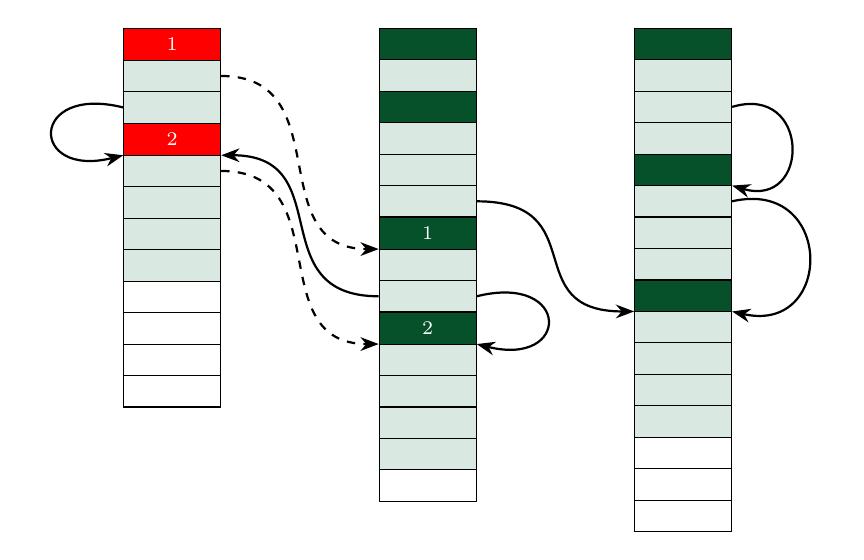
\begin{tikzpicture}[heap/.style={rectangle split, rectangle split parts=#1, draw,
        minimum width=35pt}, node distance=2cm, ->/.style={-Stealth, thick}]
    \node<1> [heap=12, rectangle split part fill={darkg, lightg, lightg,
        darkg, lightg, lightg, lightg, lightg, white}]
    (gen 0) {\color{white}{\scriptsize 1}\nodepart{four}\color{white}{\scriptsize 2}};
    \node<2> [heap=12, rectangle split part fill={red, lightg, lightg,
        darkg, lightg, lightg, lightg, lightg, white}]
    (gen 0) {\color{white}{\scriptsize 1}\nodepart{four}\color{white}{\scriptsize 2}};
    \node<3> [heap=12, rectangle split part fill={red, lightg, lightg,
        red, lightg, lightg, lightg, lightg, white}]
    (gen 0) {\color{white}{\scriptsize 1}\nodepart{four}\color{white}{\scriptsize 2}};
    \node<1>[heap=15, right = of gen 0.north east, anchor=north west,
      rectangle split part fill={darkg, lightg, darkg,
        lightg, lightg, lightg, white}] (gen 1) {};
    \node<2>[heap=15, right = of gen 0.north east, anchor=north west,
      rectangle split part fill={darkg, lightg, darkg,
        lightg, lightg, lightg, darkg, lightg, lightg, white}] (gen 1) {\nodepart{seven}\color{white}{\scriptsize 1}};
    \node<3>[heap=15, right = of gen 0.north east, anchor=north west,
      rectangle split part fill={darkg, lightg, darkg,
        lightg, lightg, lightg, darkg, lightg, lightg, darkg, lightg, lightg,
        lightg, lightg, white}] (gen 1) {\nodepart{seven}\color{white}{\scriptsize 1}\nodepart{ten}\color{white}{\scriptsize 2}};
    \node [heap=16, right = of gen 1.north east, anchor=north west,
      rectangle split part fill={darkg, lightg, lightg, lightg, darkg,
        lightg, lightg, lightg, darkg, lightg, lightg, lightg, lightg, white}]
    (gen 2) {};
    \draw[->] (gen 2.six east)..controls +(1.3, 0.3) and +(1.3, -0.3)..
    (gen 2.nine split east);
    \draw[->] (gen 2.three east)..controls +(1, 0.3) and +(1, -0.3)..
    (gen 2.five split east);
    \draw[->] (gen 1.six east)..controls +(1.5, 0) and +(-1.5, 0)..
    (gen 2.nine split west);
    \draw[->] (gen 0.three west)..controls +(-1.2, 0.3) and +(-1.2, -0.3)..
    (gen 0.four split west);
    \draw<2->[->,dashed] (gen 0.two east)..controls +(1.5, 0) and +(-1.5, 0)..
    (gen 1.seven split west);
    \draw<2>[->] (gen 1.nine west)..controls +(-1.5, 0) and +(1.5, 0)..
    (gen 0.four split east);
    \draw<3->[->,dashed] (gen 0.five east)..controls +(1.5, 0) and +(-1.5, 0)..
    (gen 1.ten split west);
    \draw<3->[->] (gen 1.nine east)..controls +(1.2, 0.3) and +(1.2, -0.3)..
    (gen 1.ten split east);
  \end{tikzpicture}
  \end{center}
\end{frame}

\begin{frame}
  \centering
  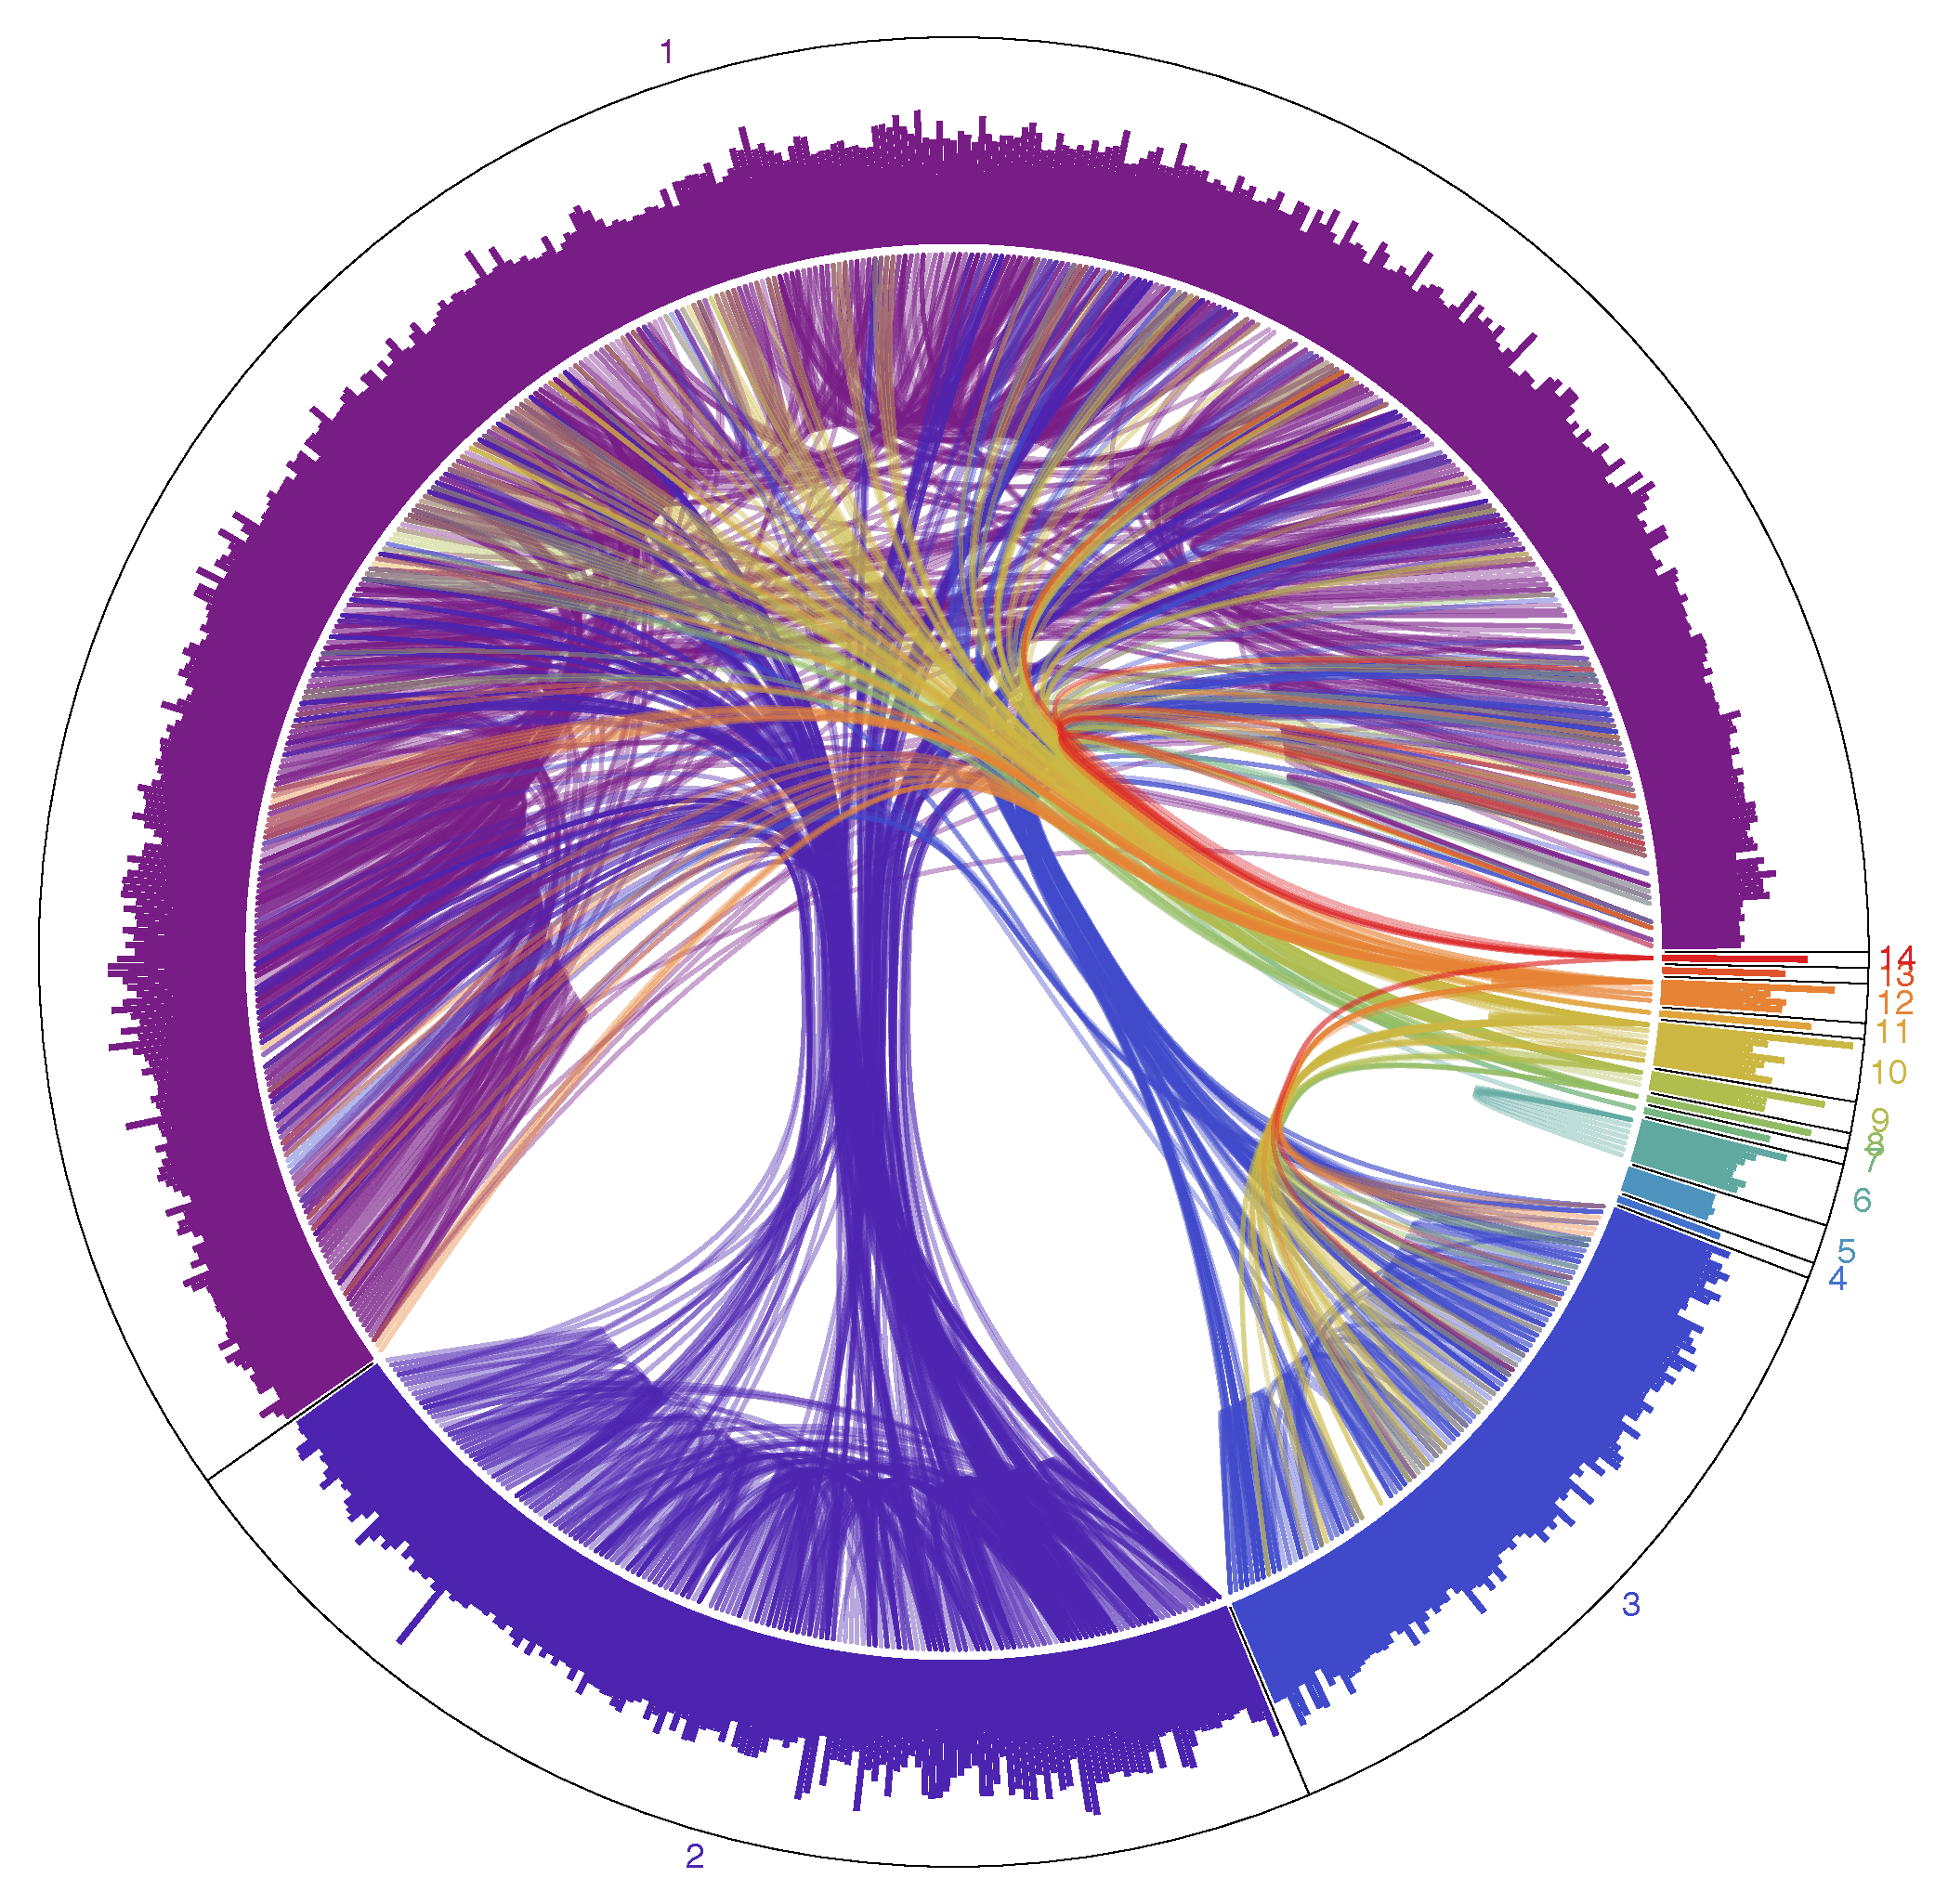
\includegraphics[height=\textheight]{certigc_theorems.pdf}
\end{frame}

\begin{frame}[fragile]{Bugs in the source C code}
  \begin{itemize}
  \item Cheney was executed too conservatively,\\ only part of
    \textsf{to} needs to be scaned.
  \pause
\item Overflow in the following calculation:\\
\begin{verbatim}
int space_size = 
        h->spaces[i].limit - h->spaces[i].start;  
\end{verbatim}
  \end{itemize}
\end{frame}

\begin{frame}[fragile]{Undefined behavior in C}
  
  \begin{itemize}
  \item Double-bounded pointer comparisons:
    \begin{Verbatim}
int Is_from(value * from_start,
            value * from_limit, value * v) {
    return (from_start <= v && v < from_limit); }
    \end{Verbatim}
    Resolved using CompCert's ``extcall\_properties''.
    \pause
  \item A classic OCaml trick:
    \begin{Verbatim}
int test_int_or_ptr (value x) {
    return (int)(((intnat)x)&1); }
    \end{Verbatim}
    Discussing \texttt{char} alignment issues with CompCert.
  \end{itemize}
\end{frame}

%\begin{frame}{A few things to note}

%\end{frame}

\section{Statistics}
\begin{frame}{Statistics}
\small
  \centering
  \rowcolors{1}{lightg}{white}
  \scalebox{1.2}{
  \begin{tabular}{|l|c|r|}\hline
    \bf{Component} & \bf{Files} & \bf{LOC} \\\hline
    Common Utilities & 10 & 2,842 \\
    Math Graph Library & 19 & 12,723\\
    Memory Model \& Logic & 13 & 2,373 \\
    Spatial Graph Library  & 10 & 6,458 \\
    Integration into VST  & 12 & 1,917 \\\hline
    Examples (excluding GC) & 13 & 3,290 \\\hline
    GC, subdivided into & 18 & 14,170 \\
%    $\bullet$ GC graphs (Math \& Spatial) & 2 & 7,382 \\
    $\bullet$ mathematical graph & 1 & 5,764 \\
    $\bullet$ spatial graph & 1 & 1,618 \\
    $\bullet$ function specifications & 1 & 461 \\
    $\bullet$ function Hoare proofs & 14 & 3,062 \\
    $\bullet$ isomorphism proof & 1 & 3,265 \\ \hline
    \bf{Total Development} & 95 & 43,773 \\\hline
  \end{tabular}}
\end{frame}

\hide{

\section{}
\begin{frame}[c]
  \centering
  \Huge
  Thank you!
\end{frame}
}

\end{document}
